\PassOptionsToPackage{unicode=true}{hyperref} % options for packages loaded elsewhere
\PassOptionsToPackage{hyphens}{url}
%
\documentclass[11pt,ignorenonframetext,]{beamer}
\usepackage{pgfpages}
\setbeamertemplate{caption}[numbered]
\setbeamertemplate{caption label separator}{: }
\setbeamercolor{caption name}{fg=normal text.fg}
\beamertemplatenavigationsymbolsempty
% Prevent slide breaks in the middle of a paragraph:
\widowpenalties 1 10000
\raggedbottom
\setbeamertemplate{part page}{
\centering
\begin{beamercolorbox}[sep=16pt,center]{part title}
  \usebeamerfont{part title}\insertpart\par
\end{beamercolorbox}
}
\setbeamertemplate{section page}{
\centering
\begin{beamercolorbox}[sep=12pt,center]{part title}
  \usebeamerfont{section title}\insertsection\par
\end{beamercolorbox}
}
\setbeamertemplate{subsection page}{
\centering
\begin{beamercolorbox}[sep=8pt,center]{part title}
  \usebeamerfont{subsection title}\insertsubsection\par
\end{beamercolorbox}
}
\AtBeginPart{
  \frame{\partpage}
}
\AtBeginSection{
  \ifbibliography
  \else
    \frame{\sectionpage}
  \fi
}
\AtBeginSubsection{
  \frame{\subsectionpage}
}
\usepackage{lmodern}
\usepackage{amssymb,amsmath}
\usepackage{ifxetex,ifluatex}
\usepackage{fixltx2e} % provides \textsubscript
\ifnum 0\ifxetex 1\fi\ifluatex 1\fi=0 % if pdftex
  \usepackage[T1]{fontenc}
  \usepackage[utf8]{inputenc}
  \usepackage{textcomp} % provides euro and other symbols
\else % if luatex or xelatex
  \usepackage{unicode-math}
  \defaultfontfeatures{Ligatures=TeX,Scale=MatchLowercase}
\fi
\usetheme[]{metropolis}
% use upquote if available, for straight quotes in verbatim environments
\IfFileExists{upquote.sty}{\usepackage{upquote}}{}
% use microtype if available
\IfFileExists{microtype.sty}{%
\usepackage[]{microtype}
\UseMicrotypeSet[protrusion]{basicmath} % disable protrusion for tt fonts
}{}
\IfFileExists{parskip.sty}{%
\usepackage{parskip}
}{% else
\setlength{\parindent}{0pt}
\setlength{\parskip}{6pt plus 2pt minus 1pt}
}
\usepackage{hyperref}
\hypersetup{
            pdftitle={Lecture 20},
            pdfauthor={Colin Rundel},
            pdfborder={0 0 0},
            breaklinks=true}
\urlstyle{same}  % don't use monospace font for urls
\newif\ifbibliography
\usepackage{color}
\usepackage{fancyvrb}
\newcommand{\VerbBar}{|}
\newcommand{\VERB}{\Verb[commandchars=\\\{\}]}
\DefineVerbatimEnvironment{Highlighting}{Verbatim}{commandchars=\\\{\}}
% Add ',fontsize=\small' for more characters per line
\newenvironment{Shaded}{}{}
\newcommand{\AlertTok}[1]{\textcolor[rgb]{1.00,0.00,0.00}{\textbf{#1}}}
\newcommand{\AnnotationTok}[1]{\textcolor[rgb]{0.38,0.63,0.69}{\textbf{\textit{#1}}}}
\newcommand{\AttributeTok}[1]{\textcolor[rgb]{0.49,0.56,0.16}{#1}}
\newcommand{\BaseNTok}[1]{\textcolor[rgb]{0.25,0.63,0.44}{#1}}
\newcommand{\BuiltInTok}[1]{#1}
\newcommand{\CharTok}[1]{\textcolor[rgb]{0.25,0.44,0.63}{#1}}
\newcommand{\CommentTok}[1]{\textcolor[rgb]{0.38,0.63,0.69}{\textit{#1}}}
\newcommand{\CommentVarTok}[1]{\textcolor[rgb]{0.38,0.63,0.69}{\textbf{\textit{#1}}}}
\newcommand{\ConstantTok}[1]{\textcolor[rgb]{0.53,0.00,0.00}{#1}}
\newcommand{\ControlFlowTok}[1]{\textcolor[rgb]{0.00,0.44,0.13}{\textbf{#1}}}
\newcommand{\DataTypeTok}[1]{\textcolor[rgb]{0.56,0.13,0.00}{#1}}
\newcommand{\DecValTok}[1]{\textcolor[rgb]{0.25,0.63,0.44}{#1}}
\newcommand{\DocumentationTok}[1]{\textcolor[rgb]{0.73,0.13,0.13}{\textit{#1}}}
\newcommand{\ErrorTok}[1]{\textcolor[rgb]{1.00,0.00,0.00}{\textbf{#1}}}
\newcommand{\ExtensionTok}[1]{#1}
\newcommand{\FloatTok}[1]{\textcolor[rgb]{0.25,0.63,0.44}{#1}}
\newcommand{\FunctionTok}[1]{\textcolor[rgb]{0.02,0.16,0.49}{#1}}
\newcommand{\ImportTok}[1]{#1}
\newcommand{\InformationTok}[1]{\textcolor[rgb]{0.38,0.63,0.69}{\textbf{\textit{#1}}}}
\newcommand{\KeywordTok}[1]{\textcolor[rgb]{0.00,0.44,0.13}{\textbf{#1}}}
\newcommand{\NormalTok}[1]{#1}
\newcommand{\OperatorTok}[1]{\textcolor[rgb]{0.40,0.40,0.40}{#1}}
\newcommand{\OtherTok}[1]{\textcolor[rgb]{0.00,0.44,0.13}{#1}}
\newcommand{\PreprocessorTok}[1]{\textcolor[rgb]{0.74,0.48,0.00}{#1}}
\newcommand{\RegionMarkerTok}[1]{#1}
\newcommand{\SpecialCharTok}[1]{\textcolor[rgb]{0.25,0.44,0.63}{#1}}
\newcommand{\SpecialStringTok}[1]{\textcolor[rgb]{0.73,0.40,0.53}{#1}}
\newcommand{\StringTok}[1]{\textcolor[rgb]{0.25,0.44,0.63}{#1}}
\newcommand{\VariableTok}[1]{\textcolor[rgb]{0.10,0.09,0.49}{#1}}
\newcommand{\VerbatimStringTok}[1]{\textcolor[rgb]{0.25,0.44,0.63}{#1}}
\newcommand{\WarningTok}[1]{\textcolor[rgb]{0.38,0.63,0.69}{\textbf{\textit{#1}}}}
\usepackage{longtable,booktabs}
\usepackage{caption}
% These lines are needed to make table captions work with longtable:
\makeatletter
\def\fnum@table{\tablename~\thetable}
\makeatother
\setlength{\emergencystretch}{3em}  % prevent overfull lines
\providecommand{\tightlist}{%
  \setlength{\itemsep}{0pt}\setlength{\parskip}{0pt}}
\setcounter{secnumdepth}{0}

% set default figure placement to htbp
\makeatletter
\def\fps@figure{htbp}
\makeatother

\usepackage{geometry}
\usepackage{graphicx}

\usepackage{bbold}
\usepackage{lmodern}


\usepackage{url}		% produces hyperlinks

\usepackage{colortbl}	% allows for color usage in tables
\usepackage{multirow}	% allows for rows that span multiple rows in tables

\usepackage{color}          	% gives color options
\usepackage{xcolor}		% this package has a variety of color options

\usepackage{multicol}
\usepackage{textcomp}

\usepackage{setspace}
\usepackage{changepage}
\usepackage{isotope}

\singlespacing

\def\begincol{\begin{column}}
\def\endcol{\end{column}}

\def\begincols{\begin{columns}}
\def\endcols{\end{columns}}

%%%%%%%%%%%%%%%%
% Small code output
%%%%%%%%%%%%%%%%

%% change fontsize of R code

\makeatletter
\@ifundefined{Shaded}{\newenvironment{Shaded}{}{}}{}
\makeatother


\let\oldShaded\Shaded
\let\endoldShaded\endShaded
\renewenvironment{Shaded}{\footnotesize\begin{spacing}{0.9}\oldShaded}{\endoldShaded\end{spacing}}

%% change fontsize of output
\let\oldverbatim\verbatim
\let\endoldverbatim\endverbatim
\renewenvironment{verbatim}{\footnotesize\begin{spacing}{0.9}\oldverbatim}{\endoldverbatim\end{spacing}}


\newcommand{\tinyoutput}{
  \renewenvironment{Shaded}{\tiny\begin{spacing}{0.9}\oldShaded}{\endoldShaded\end{spacing}}
  \renewenvironment{verbatim}{\tiny\begin{spacing}{0.9}\oldverbatim}{\endoldverbatim\end{spacing}}
}

\newcommand{\scriptoutput}{
  \renewenvironment{Shaded}{\scriptsize\begin{spacing}{0.9}\oldShaded}{\endoldShaded\end{spacing}}
  \renewenvironment{verbatim}{\scriptsize\begin{spacing}{0.9}\oldverbatim}{\endoldverbatim\end{spacing}}
}

\newcommand{\footnoteoutput}{
  \renewenvironment{Shaded}{\footnotesize\begin{spacing}{0.9}\oldShaded}{\endoldShaded\end{spacing}}
  \renewenvironment{verbatim}{\footnotesize\begin{spacing}{0.9}\oldverbatim}{\endoldverbatim\end{spacing}}
}

%\newcommand{\verbatimfont}[1]{\renewcommand{\verbatim@font}{\ttfamily#1}}


%%%%%%%%%%%%%%%%
% Custom Colors
%%%%%%%%%%%%%%%%

\definecolor{redhl}{rgb}{0.98,0.29,0.28}
\definecolor{yellowhl}{rgb}{0.98,0.87,0.28}


\xdefinecolor{oiBlue}{rgb}{0.15, 0.35, 0.55}
\xdefinecolor{gray}{rgb}{0.5, 0.5, 0.5}
\xdefinecolor{darkGray}{rgb}{0.3, 0.3, 0.3}
\xdefinecolor{darkerGray}{rgb}{0.2, 0.2, 0.2}
\xdefinecolor{rubineRed}{rgb}{0.89,0,0.30}
\xdefinecolor{linkCol}{rgb}{0.11,0.49,0.95}	
\xdefinecolor{irishGreen}{rgb}{0,0.60,0}	
\xdefinecolor{darkturquoise}{rgb}{0.44, 0.58, 0.86}
\definecolor{lightGreen}{rgb}{0.533,0.765,0.42}
%\xdefinecolor{hlblue}{rgb}{0.051,0.65,1}
\xdefinecolor{hlblue}{rgb}{ 0.055, 0.639, 0.831}
\definecolor{light}{rgb}{.337,.608,.741}
\definecolor{dark}{rgb}{.337,.608,.741}

\definecolor{cpink}{rgb}{0.93, 0.23, 0.51}

%%%%%%%%%%%%%%%%
% Custom Commands
%%%%%%%%%%%%%%%%

% text colors
\newcommand{\red}[1]{\textit{\textcolor{rubineRed}{#1}}}
\newcommand{\orange}[1]{\textit{\textcolor{orange}{#1}}}
\newcommand{\pink}[1]{\textit{\textcolor{rubineRed!90!white!50}{#1}}}
\newcommand{\green}[1]{\textit{\textcolor{irishGreen}{#1}}}
\newcommand{\blue}[1]{\textit{\textcolor{darkturquoise}{#1}}}
\newcommand{\light}[1]{\textcolor{light}{\textbf{#1}}}
\newcommand{\dark}[1]{\textcolor{dark}{#1}}
\newcommand{\gray}[1]{\textcolor{gray}{#1}}


% mail
\newcommand{\mail}[1]{\href{mailto:#1}{\textit{\textcolor{linkCol}{#1}}}}

% highlighting: hl, hlGr, mathhl
\newcommand{\hl}[1]{\textit{\textcolor{hlblue}{#1}}}
\newcommand{\hlGr}[1]{\textit{\textcolor{lightGreen}{#1}}}
\newcommand{\hlRd}[1]{\textit{\textcolor{rubineRed}{#1}}}
\newcommand{\mathhl}[1]{\textcolor{hlblue}{\ensuremath{#1}}}
\newcommand{\hlr}[1]{\fcolorbox{redhl}{white}{$\displaystyle #1$}}
\newcommand{\hly}[1]{\fcolorbox{yellowhl}{white}{$\displaystyle #1$}}


\newcommand{\vvfill}{\vskip0pt plus 1filll}

\DeclareMathOperator*{\argmin}{arg\,min}
\DeclareMathOperator*{\argmax}{arg\,max}

\title{Lecture 20}
\providecommand{\subtitle}[1]{}
\subtitle{Point referenced data (pt. 2)}
\author{Colin Rundel}
\date{11/14/2018}

\begin{document}
\frame{\titlepage}

\hypertarget{loa-loa-example}{%
\section{Loa Loa Example}\label{loa-loa-example}}

\begin{frame}{Loa Loa}
\protect\hypertarget{loa-loa}{}

\begin{center}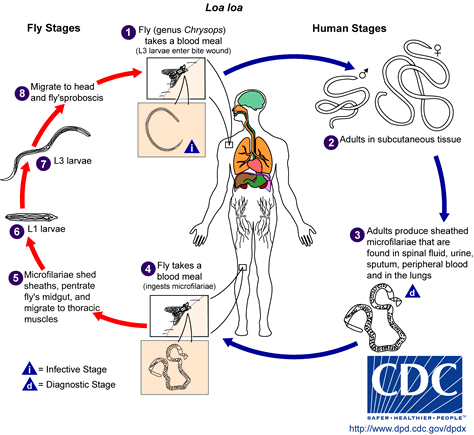
\includegraphics[width=0.7\textwidth]{figs/loa_loa_LifeCycle} \end{center}

\end{frame}

\begin{frame}[fragile]{Data}
\protect\hypertarget{data}{}

\begin{Shaded}
\begin{Highlighting}[]
\NormalTok{loaloa =}\StringTok{ }\KeywordTok{tbl_df}\NormalTok{(PrevMap}\OperatorTok{::}\NormalTok{loaloa) }\OperatorTok\StringTok{ }\KeywordTok{setNames}\NormalTok{(., }\KeywordTok{tolower}\NormalTok{(}\KeywordTok{names}\NormalTok{(.))) }\OperatorTok
\StringTok{  }\KeywordTok{rename}\NormalTok{(}\DataTypeTok{elev=}\NormalTok{elevation)}

\NormalTok{loaloa}
\CommentTok{## # A tibble: 197 x 11}
\CommentTok{##      row villcode longitude latitude no_exam no_inf  elev mean9901 max9901}
\CommentTok{##    <int>    <int>     <dbl>    <dbl>   <int>  <int> <int>    <dbl>   <dbl>}
\CommentTok{##  1     1      214      8.04     5.74     162      0   108    0.439    0.69}
\CommentTok{##  2     2      215      8.00     5.68     167      1    99    0.426    0.74}
\CommentTok{##  3     3      118      8.91     5.35      88      5   783    0.491    0.79}
\CommentTok{##  4     4      219      8.10     5.92      62      5   104    0.432    0.67}
\CommentTok{##  5     5      212      8.18     5.10     167      3   109    0.415    0.85}
\CommentTok{##  6     6      116      8.93     5.36      66      3   909    0.436    0.8 }
\CommentTok{##  7     7       16     11.4      4.88     163     11   503    0.502    0.78}
\CommentTok{##  8     8      217      8.07     5.90      83      0   103    0.373    0.69}
\CommentTok{##  9     9      112      9.02     5.59      30      4   751    0.481    0.8 }
\CommentTok{## 10    10      104      9.31     6.00      57      4   268    0.487    0.84}
\CommentTok{## # ... with 187 more rows, and 2 more variables: min9901 <dbl>,}
\CommentTok{## #   stdev9901 <dbl>}
\end{Highlighting}
\end{Shaded}

\end{frame}

\begin{frame}{Spatial Distribution}
\protect\hypertarget{spatial-distribution}{}

\begin{center}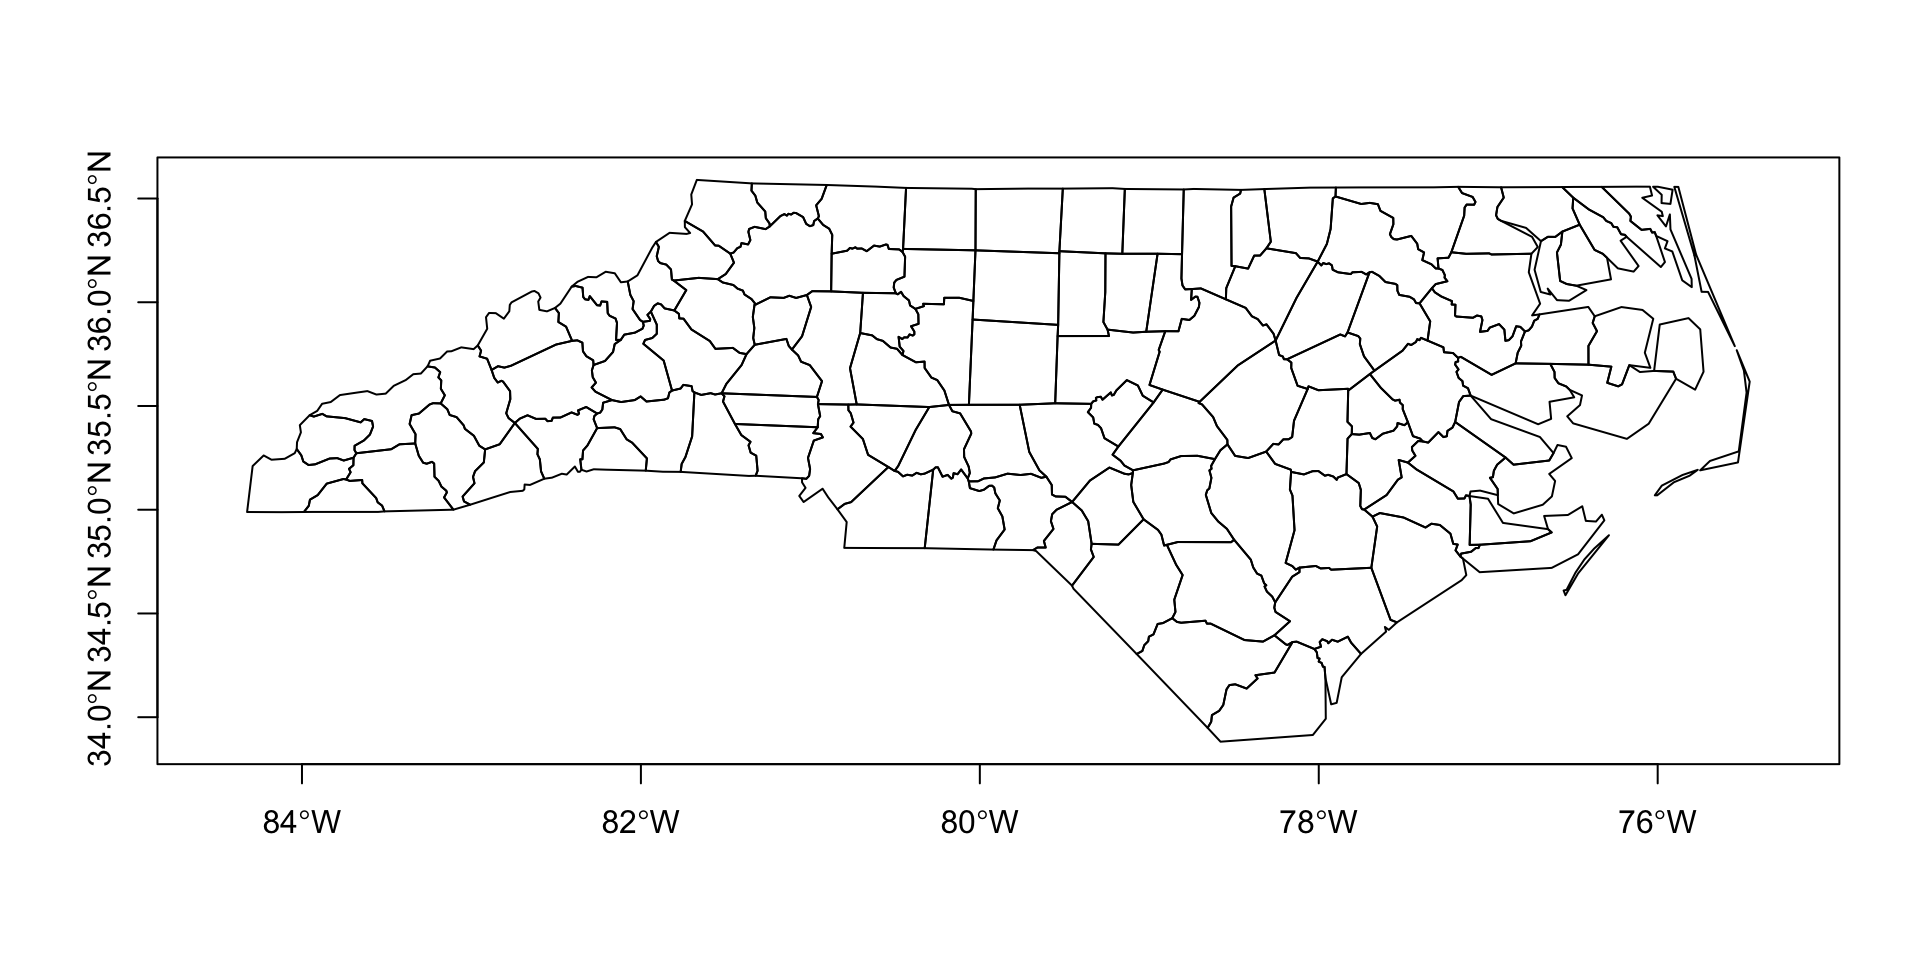
\includegraphics[width=0.9\textwidth]{Lec20_files/figure-beamer/unnamed-chunk-3-1} \end{center}

\end{frame}

\begin{frame}[t]{Normalized Difference Vegetation Index (NDVI)}
\protect\hypertarget{normalized-difference-vegetation-index-ndvi}{}

\vspace{-2.5mm}

\begin{center}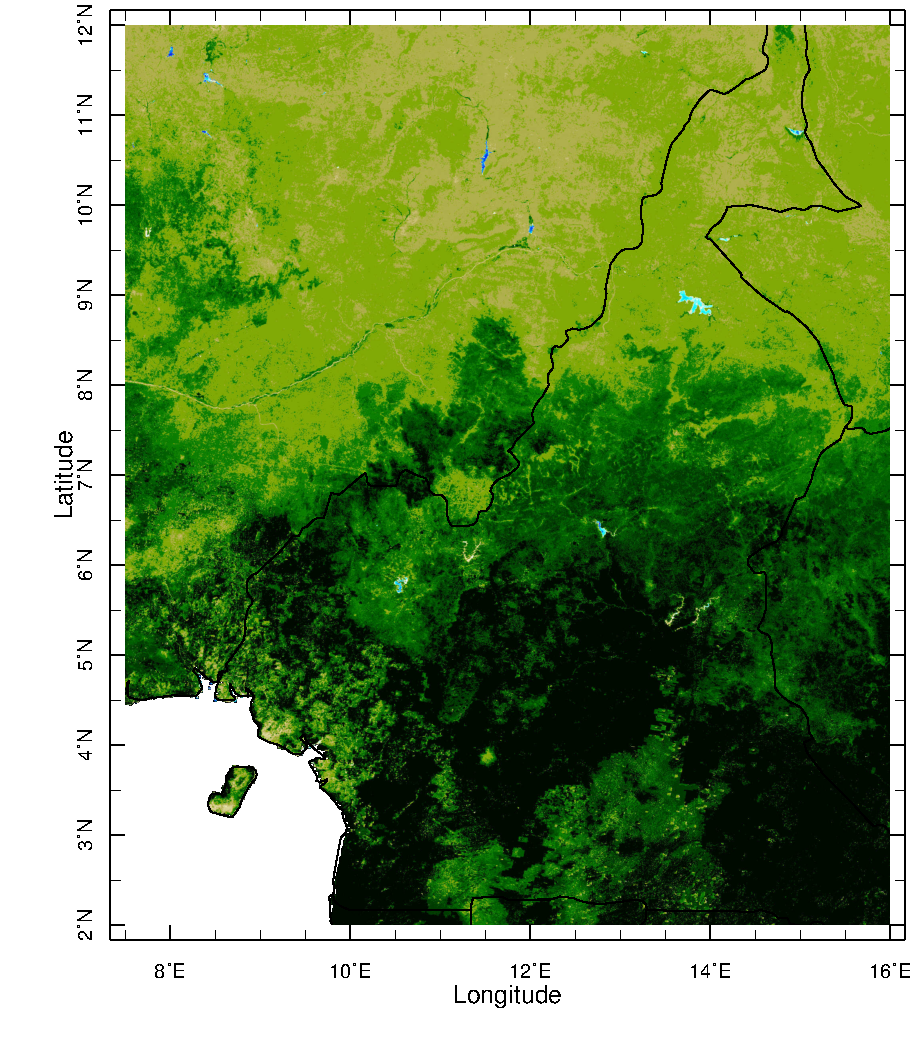
\includegraphics[width=0.6\textwidth]{figs/ndvi_cameroon} \end{center}

\begin{center}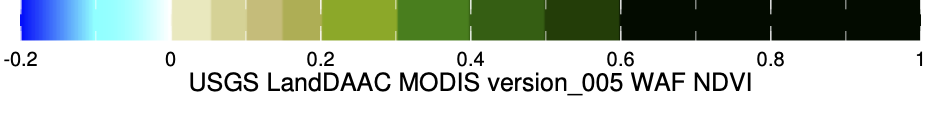
\includegraphics[width=0.6\textwidth]{figs/ndvi_cameroon_scale} \end{center}

\end{frame}

\begin{frame}[fragile]{Paper / Data summary}
\protect\hypertarget{paper-data-summary}{}

Original paper - Diggle, et. al.~(2007). \emph{Spatial modelling and
prediction of Loa loa risk: decision making under uncertainty}. Annals
of Tropical Medicine and Parasitology, 101, 499-509.

\vspace{4mm}

\begin{itemize}
\tightlist
\item
  \texttt{no\_exam} and \texttt{no\_inf} - Collected between 1991 and
  2001 by NGOs (original paper mentions 168 villages and 21,938
  observations)
\end{itemize}

\vspace{2mm}

\begin{itemize}
\tightlist
\item
  \texttt{elev} - USGS gtopo30 (1km resolution)
\end{itemize}

\vspace{2mm}

\begin{itemize}
\tightlist
\item
  \texttt{mean9901} to \texttt{stdev9901} - aggregated data from 1999 to
  2001 from the Flemish Institute for Technological Research (1 km
  resolution)
\end{itemize}

\end{frame}

\begin{frame}{Diggle's Model}
\protect\hypertarget{diggles-model}{}

\[ 
\begin{aligned}
\log \left( \frac{p(s)}{1-p(s)} \right) = \alpha &+ f_1(\text{elev}(s)) \\
&+ f_2(\text{MAX.NDVI}(s)) \\
&+ f_3(\text{SD.NDVI}(s)) + w(s) 
\end{aligned}
\]

where

\[ w(s) \sim \mathcal{N}(0, \Sigma) \]
\[ \{\Sigma\}_{ij} = \sigma^2 \, \exp(-d \,\phi) \]

\end{frame}

\begin{frame}{EDA}
\protect\hypertarget{eda}{}

\begin{center}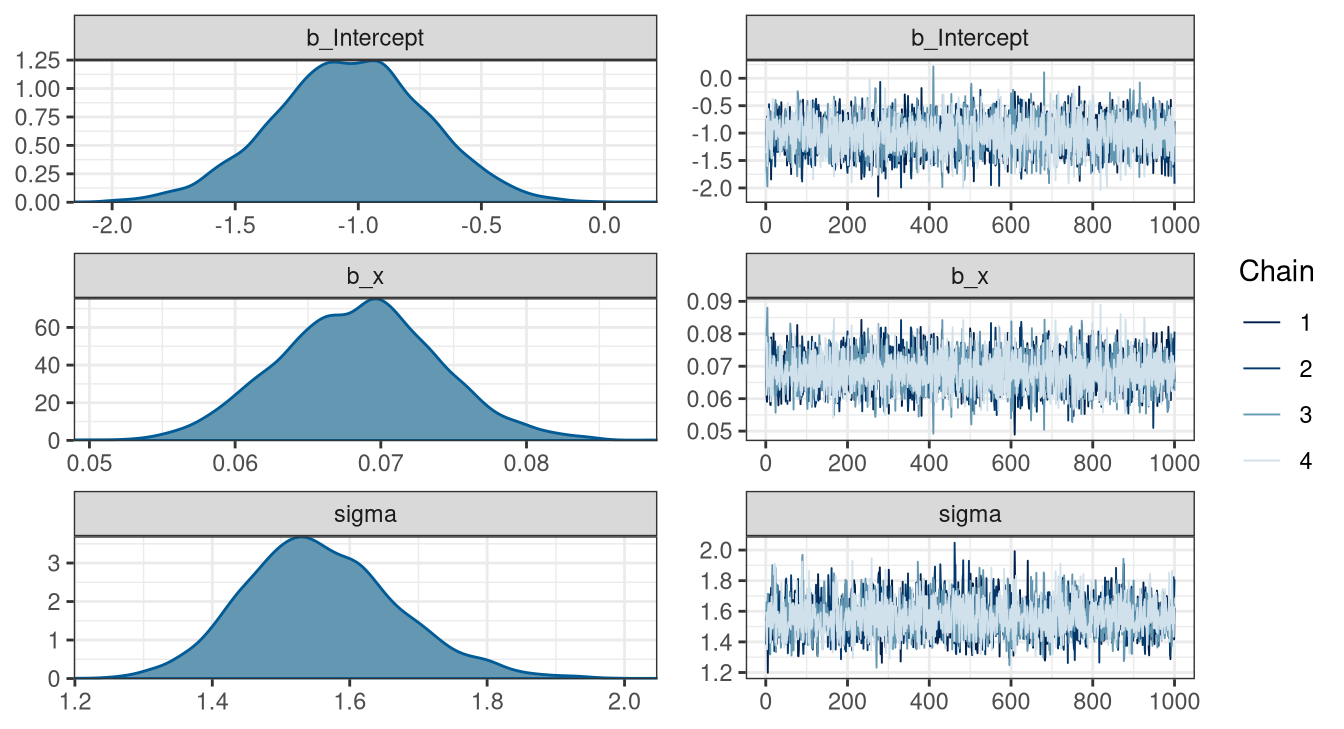
\includegraphics[width=0.8\textwidth]{Lec20_files/figure-beamer/unnamed-chunk-5-1} \end{center}

\end{frame}

\begin{frame}{Diggle's EDA}
\protect\hypertarget{diggles-eda}{}

\begin{center}
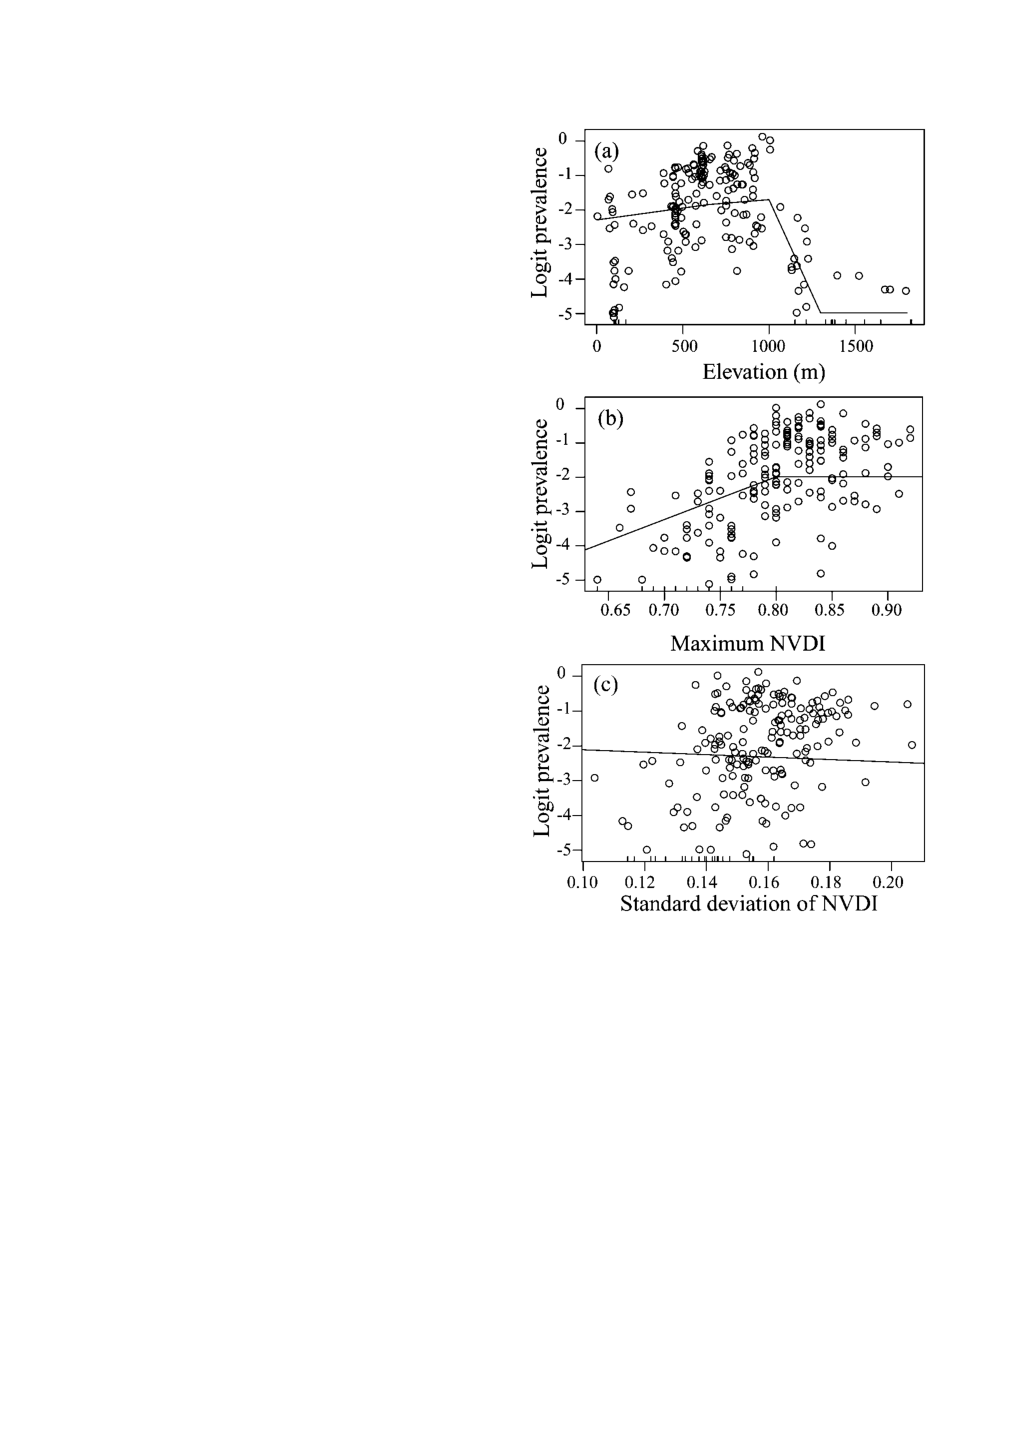
\includegraphics[width=0.65\textwidth]{figs/diggle_eda.pdf} \\
\end{center}

\end{frame}

\begin{frame}[fragile,t]{Data Augmentation}
\protect\hypertarget{data-augmentation}{}

\begin{Shaded}
\begin{Highlighting}[]
\NormalTok{loaloa =}\StringTok{ }\NormalTok{loaloa }\OperatorTok\StringTok{ }
\StringTok{  }\KeywordTok{mutate}\NormalTok{(}
    \DataTypeTok{elev_f =} \KeywordTok{cut}\NormalTok{(elev, }\DataTypeTok{breaks=}\KeywordTok{c}\NormalTok{(}\DecValTok{0}\NormalTok{,}\DecValTok{1000}\NormalTok{,}\DecValTok{1300}\NormalTok{,}\DecValTok{2000}\NormalTok{), }\DataTypeTok{dig.lab=}\DecValTok{5}\NormalTok{),}
    \DataTypeTok{max_f  =} \KeywordTok{cut}\NormalTok{(max9901, }\DataTypeTok{breaks=}\KeywordTok{c}\NormalTok{(}\DecValTok{0}\NormalTok{,}\FloatTok{0.8}\NormalTok{,}\DecValTok{1}\NormalTok{))}
\NormalTok{  )}

\NormalTok{loaloa }\OperatorTok\StringTok{ }\KeywordTok{select}\NormalTok{(elev, elev_f, max9901, max_f)}
\CommentTok{## # A tibble: 197 x 4}
\CommentTok{##     elev elev_f   max9901 max_f  }
\CommentTok{##    <int> <fct>      <dbl> <fct>  }
\CommentTok{##  1   108 (0,1000]    0.69 (0,0.8]}
\CommentTok{##  2    99 (0,1000]    0.74 (0,0.8]}
\CommentTok{##  3   783 (0,1000]    0.79 (0,0.8]}
\CommentTok{##  4   104 (0,1000]    0.67 (0,0.8]}
\CommentTok{##  5   109 (0,1000]    0.85 (0.8,1]}
\CommentTok{##  6   909 (0,1000]    0.8  (0,0.8]}
\CommentTok{##  7   503 (0,1000]    0.78 (0,0.8]}
\CommentTok{##  8   103 (0,1000]    0.69 (0,0.8]}
\CommentTok{##  9   751 (0,1000]    0.8  (0,0.8]}
\CommentTok{## 10   268 (0,1000]    0.84 (0.8,1]}
\CommentTok{## # ... with 187 more rows}
\end{Highlighting}
\end{Shaded}

\end{frame}

\begin{frame}[fragile]{Model Matrix \{.\}}
\protect\hypertarget{model-matrix-.}{}

\scriptoutput

\begin{Shaded}
\begin{Highlighting}[]
\KeywordTok{model.matrix}\NormalTok{(}
  \OperatorTok{~}\StringTok{ }\NormalTok{elev}\OperatorTok{:}\NormalTok{elev_f }\OperatorTok{-}\StringTok{ }\DecValTok{1}\NormalTok{, }
  \DataTypeTok{data =}\NormalTok{ loaloa}
\NormalTok{) }\OperatorTok
\StringTok{  }\KeywordTok{as_data_frame}\NormalTok{()}
\CommentTok{## # A tibble: 197 x 3}
\CommentTok{##    `elev:elev_f(0,1000]` `elev:elev_f(1000,1300]` `elev:elev_f(1300,2000]`}
\CommentTok{##                    <dbl>                    <dbl>                    <dbl>}
\CommentTok{##  1                   108                        0                        0}
\CommentTok{##  2                    99                        0                        0}
\CommentTok{##  3                   783                        0                        0}
\CommentTok{##  4                   104                        0                        0}
\CommentTok{##  5                   109                        0                        0}
\CommentTok{##  6                   909                        0                        0}
\CommentTok{##  7                   503                        0                        0}
\CommentTok{##  8                   103                        0                        0}
\CommentTok{##  9                   751                        0                        0}
\CommentTok{## 10                   268                        0                        0}
\CommentTok{## # ... with 187 more rows}
\end{Highlighting}
\end{Shaded}

\end{frame}

\begin{frame}[fragile]{OOS Validation}
\protect\hypertarget{oos-validation}{}

\begin{Shaded}
\begin{Highlighting}[]
\NormalTok{loaloa_test =}\StringTok{ }\NormalTok{loaloa }\OperatorTok\StringTok{ }\KeywordTok{sample_frac}\NormalTok{(}\FloatTok{0.20}\NormalTok{)}
\NormalTok{loaloa =}\StringTok{ }\KeywordTok{anti_join}\NormalTok{(loaloa, loaloa_test, }\DataTypeTok{quiet=}\OtherTok{TRUE}\NormalTok{)}
\end{Highlighting}
\end{Shaded}

\begin{center}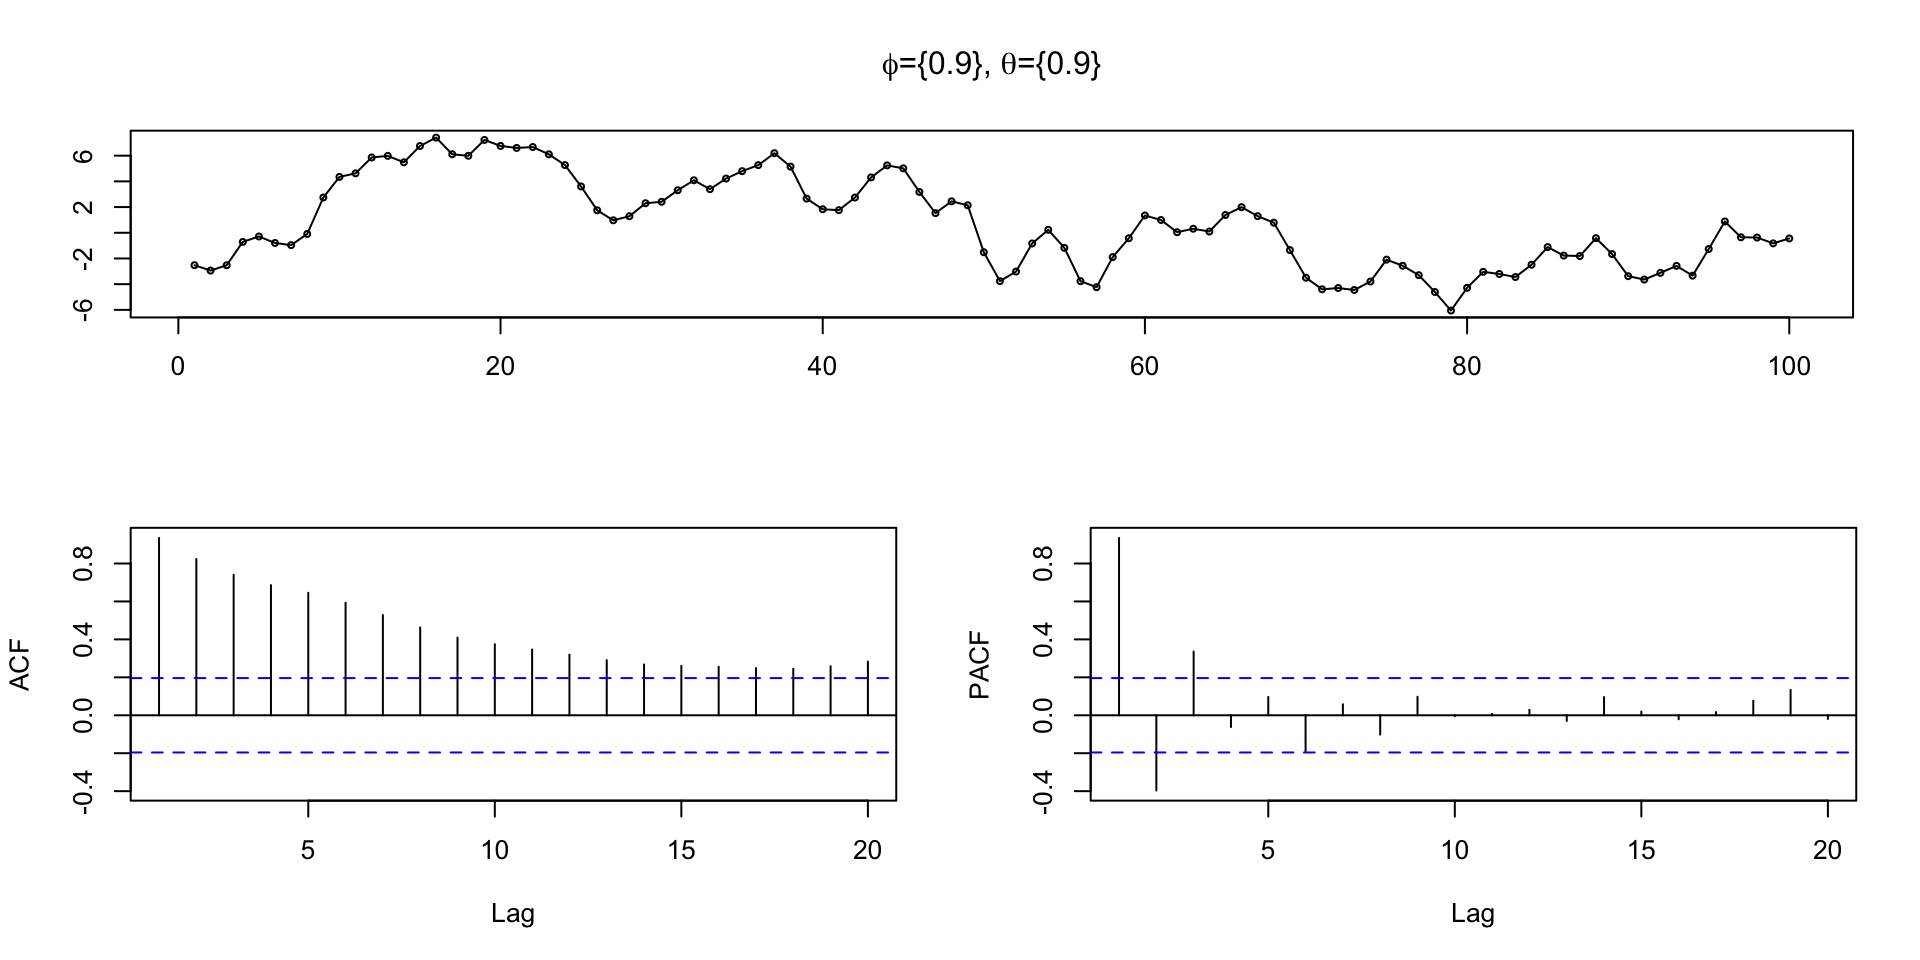
\includegraphics[width=0.95\textwidth]{Lec20_files/figure-beamer/unnamed-chunk-9-1} \end{center}

\end{frame}

\begin{frame}[fragile]{Model}
\protect\hypertarget{model}{}

\scriptoutput

\begin{Shaded}
\begin{Highlighting}[]
\NormalTok{g =}\StringTok{ }\KeywordTok{glm}\NormalTok{(no_inf}\OperatorTok{/}\NormalTok{no_exam }\OperatorTok{~}\StringTok{ }\NormalTok{elev}\OperatorTok{:}\NormalTok{elev_f }\OperatorTok{+}\StringTok{ }\NormalTok{max9901}\OperatorTok{:}\NormalTok{max_f }\OperatorTok{+}\StringTok{ }\NormalTok{stdev9901, }
        \DataTypeTok{data=}\NormalTok{loaloa, }\DataTypeTok{family=}\NormalTok{binomial, }\DataTypeTok{weights=}\NormalTok{loaloa}\OperatorTok{$}\NormalTok{no_exam)}

\KeywordTok{summary}\NormalTok{(g)}
\CommentTok{## }
\CommentTok{## Call:}
\CommentTok{## glm(formula = no_inf/no_exam ~ elev:elev_f + max9901:max_f + }
\CommentTok{##     stdev9901, family = binomial, data = loaloa, weights = loaloa$no_exam)}
\CommentTok{## }
\CommentTok{## Deviance Residuals: }
\CommentTok{##     Min       1Q   Median       3Q      Max  }
\CommentTok{## -6.9522  -2.5662  -0.4621   1.6720  10.1809  }
\CommentTok{## }
\CommentTok{## Coefficients:}
\CommentTok{##                          Estimate Std. Error z value Pr(>|z|)    }
\CommentTok{## (Intercept)            -8.5735389  0.5333413 -16.075  < 2e-16 ***}
\CommentTok{## stdev9901              11.9141737  1.3070028   9.116  < 2e-16 ***}
\CommentTok{## elev:elev_f(0,1000]     0.0015951  0.0001018  15.660  < 2e-16 ***}
\CommentTok{## elev:elev_f(1000,1300]  0.0003343  0.0000953   3.507 0.000453 ***}
\CommentTok{## elev:elev_f(1300,2000] -0.0016964  0.0002513  -6.750 1.48e-11 ***}
\CommentTok{## max9901:max_f(0,0.8]    5.2697375  0.6918702   7.617 2.60e-14 ***}
\CommentTok{## max9901:max_f(0.8,1]    5.2632126  0.6362108   8.273  < 2e-16 ***}
\CommentTok{## ---}
\CommentTok{## Signif. codes:  0 '***' 0.001 '**' 0.01 '*' 0.05 '.' 0.1 ' ' 1}
\CommentTok{## }
\CommentTok{## (Dispersion parameter for binomial family taken to be 1)}
\CommentTok{## }
\CommentTok{##     Null deviance: 3210.2  on 157  degrees of freedom}
\CommentTok{## Residual deviance: 1557.4  on 151  degrees of freedom}
\CommentTok{## AIC: 2181}
\CommentTok{## }
\CommentTok{## Number of Fisher Scoring iterations: 5}
\end{Highlighting}
\end{Shaded}

\end{frame}

\begin{frame}{Predictions - Training}
\protect\hypertarget{predictions---training}{}

\begin{center}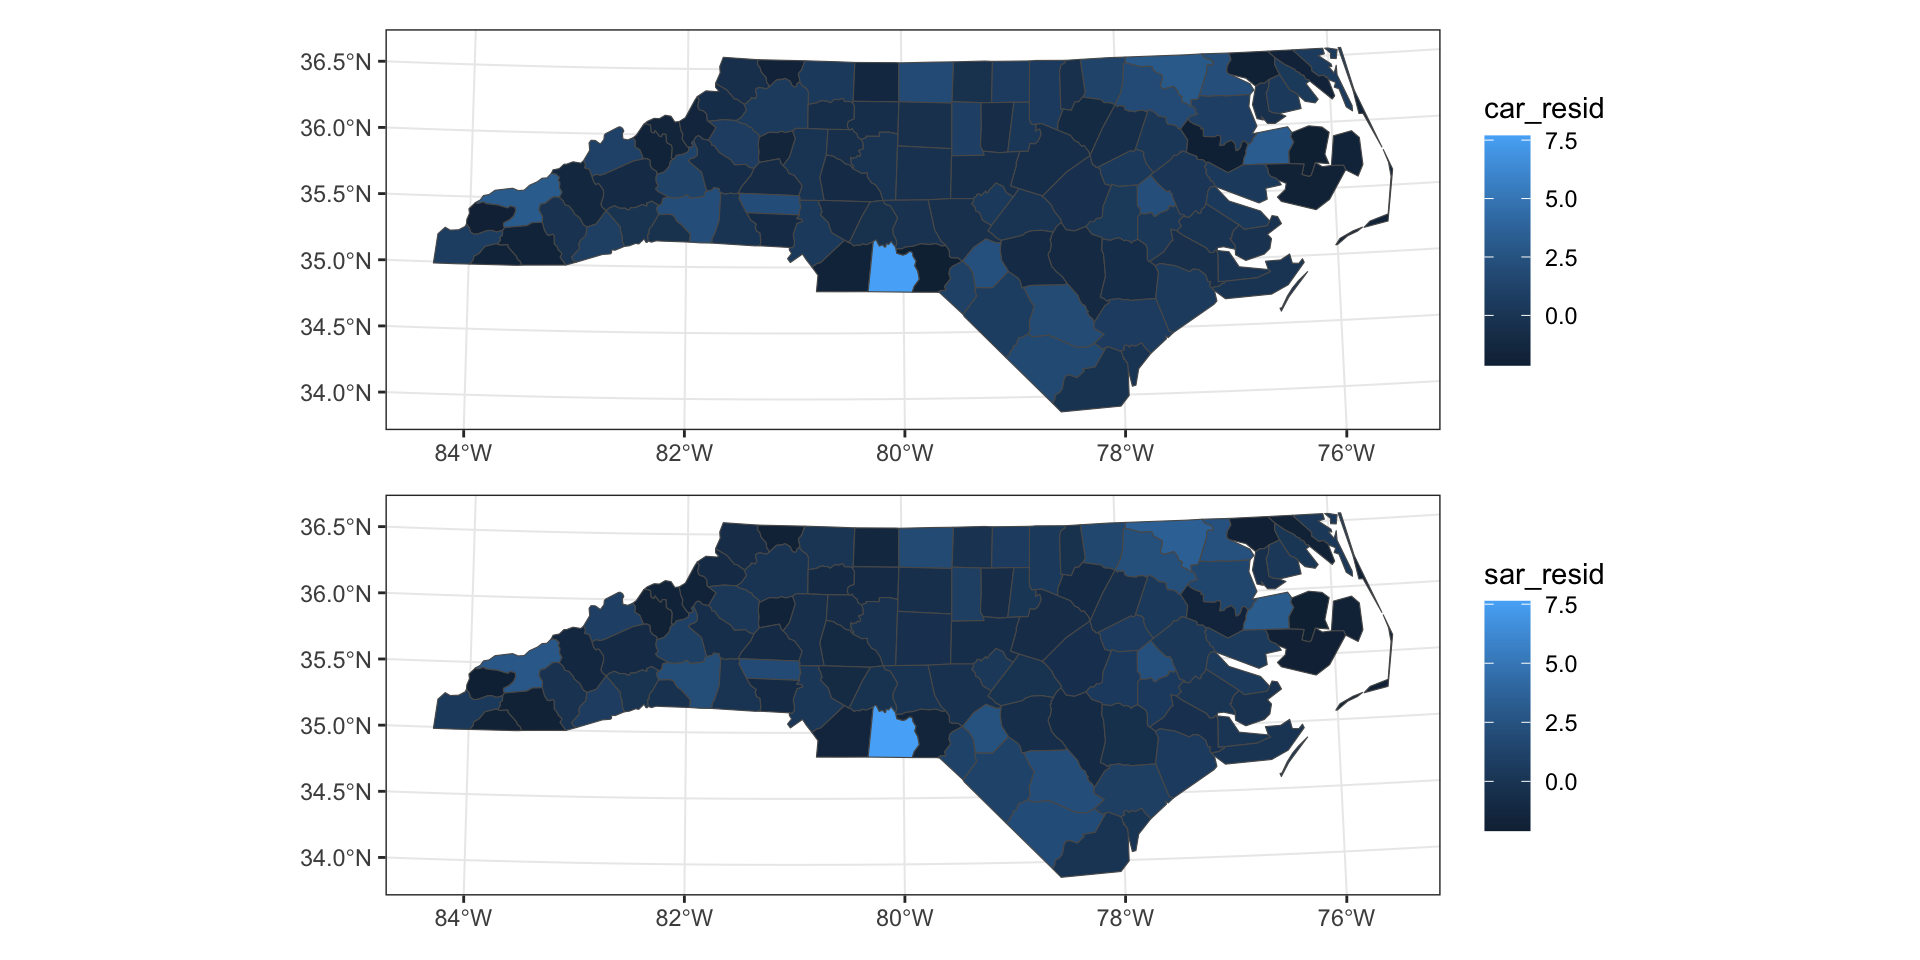
\includegraphics[width=\textwidth]{Lec20_files/figure-beamer/unnamed-chunk-12-1} \end{center}

\end{frame}

\begin{frame}{Predictions - Testing}
\protect\hypertarget{predictions---testing}{}

\begin{center}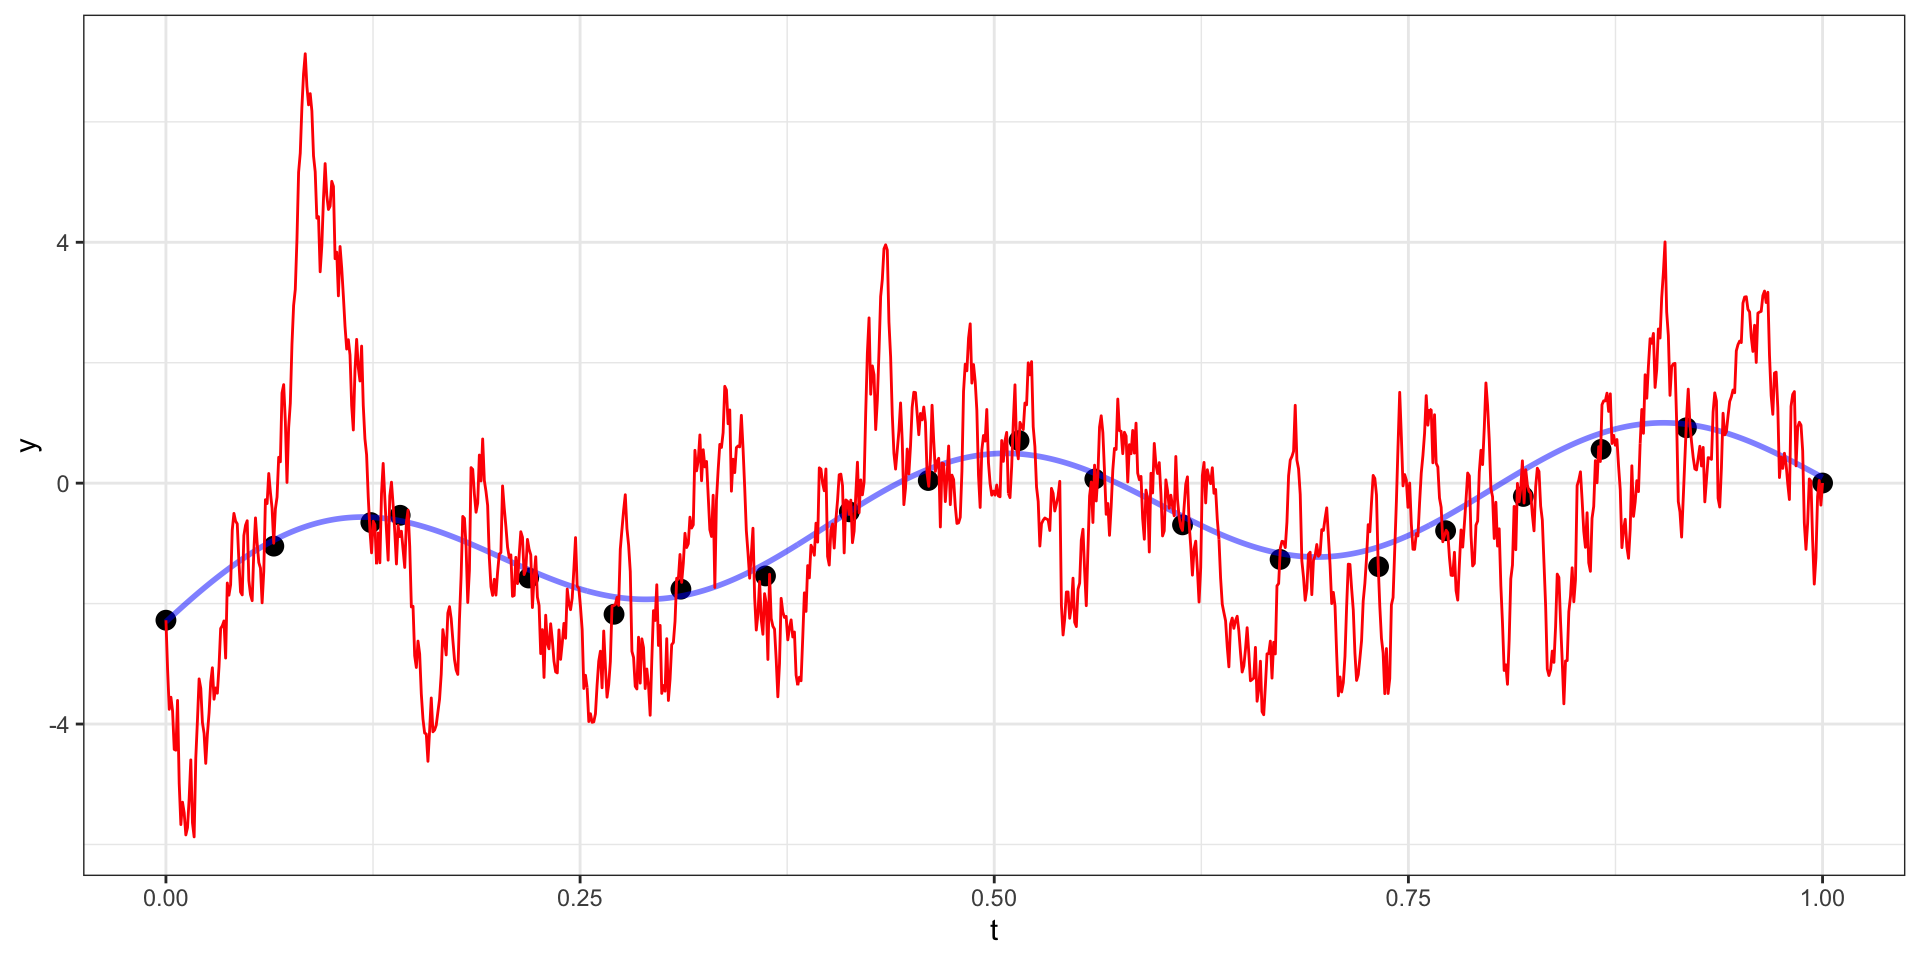
\includegraphics[width=\textwidth]{Lec20_files/figure-beamer/unnamed-chunk-13-1} \end{center}

\end{frame}

\begin{frame}{Fit - Training}
\protect\hypertarget{fit---training}{}

\scriptoutput

\begin{center}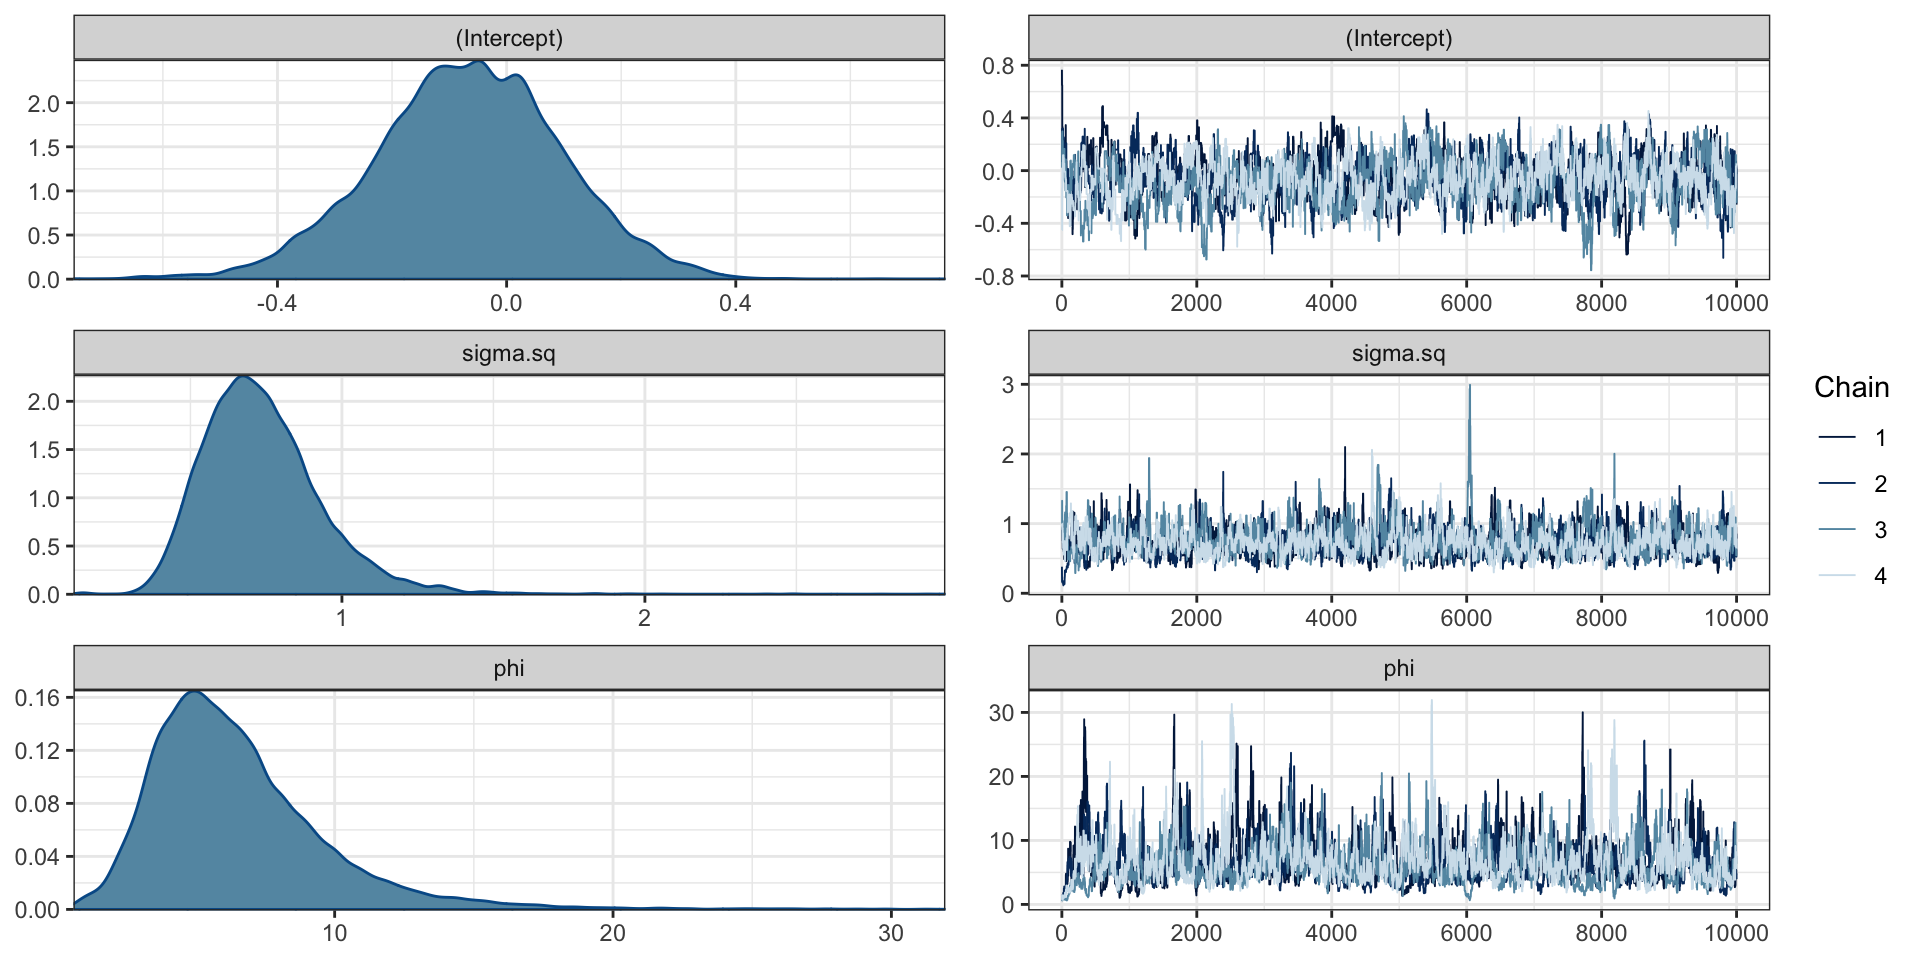
\includegraphics[width=\textwidth]{Lec20_files/figure-beamer/unnamed-chunk-14-1} \end{center}

\end{frame}

\begin{frame}{Fit - Testing}
\protect\hypertarget{fit---testing}{}

\scriptoutput

\begin{center}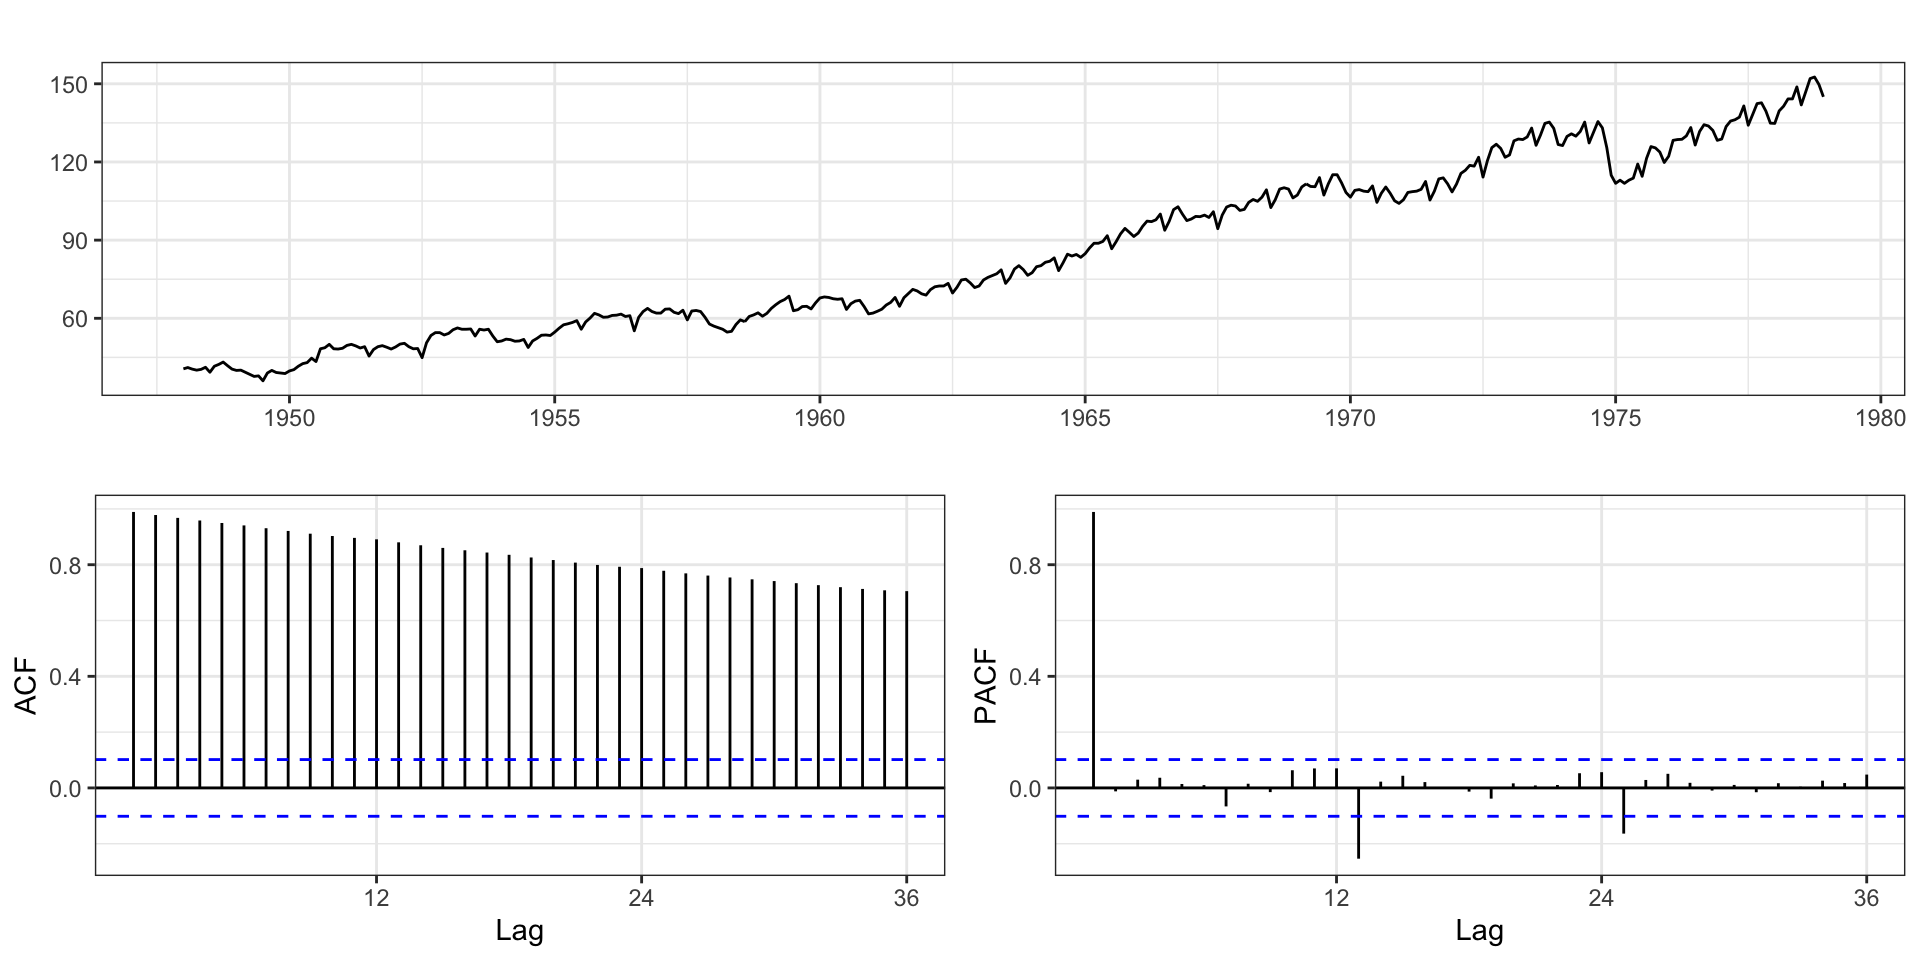
\includegraphics[width=\textwidth]{Lec20_files/figure-beamer/unnamed-chunk-15-1} \end{center}

\end{frame}

\begin{frame}[fragile]{Spatial Structure?}
\protect\hypertarget{spatial-structure}{}

\begin{Shaded}
\begin{Highlighting}[]
\NormalTok{geoR}\OperatorTok{::}\KeywordTok{variog}\NormalTok{(}\DataTypeTok{coords =} \KeywordTok{cbind}\NormalTok{(loaloa}\OperatorTok{$}\NormalTok{longitude, loaloa}\OperatorTok{$}\NormalTok{latitude), }
       \DataTypeTok{data =}\NormalTok{ loaloa}\OperatorTok{$}\NormalTok{prop }\OperatorTok{-}\StringTok{ }\NormalTok{loaloa}\OperatorTok{$}\NormalTok{glm_pred,}
       \DataTypeTok{uvec =} \KeywordTok{seq}\NormalTok{(}\DecValTok{0}\NormalTok{, }\DecValTok{4}\NormalTok{, }\DataTypeTok{length.out =} \DecValTok{50}\NormalTok{)) }\OperatorTok\StringTok{ }\KeywordTok{plot}\NormalTok{()}
\CommentTok{## variog: computing omnidirectional variogram}
\end{Highlighting}
\end{Shaded}

\begin{center}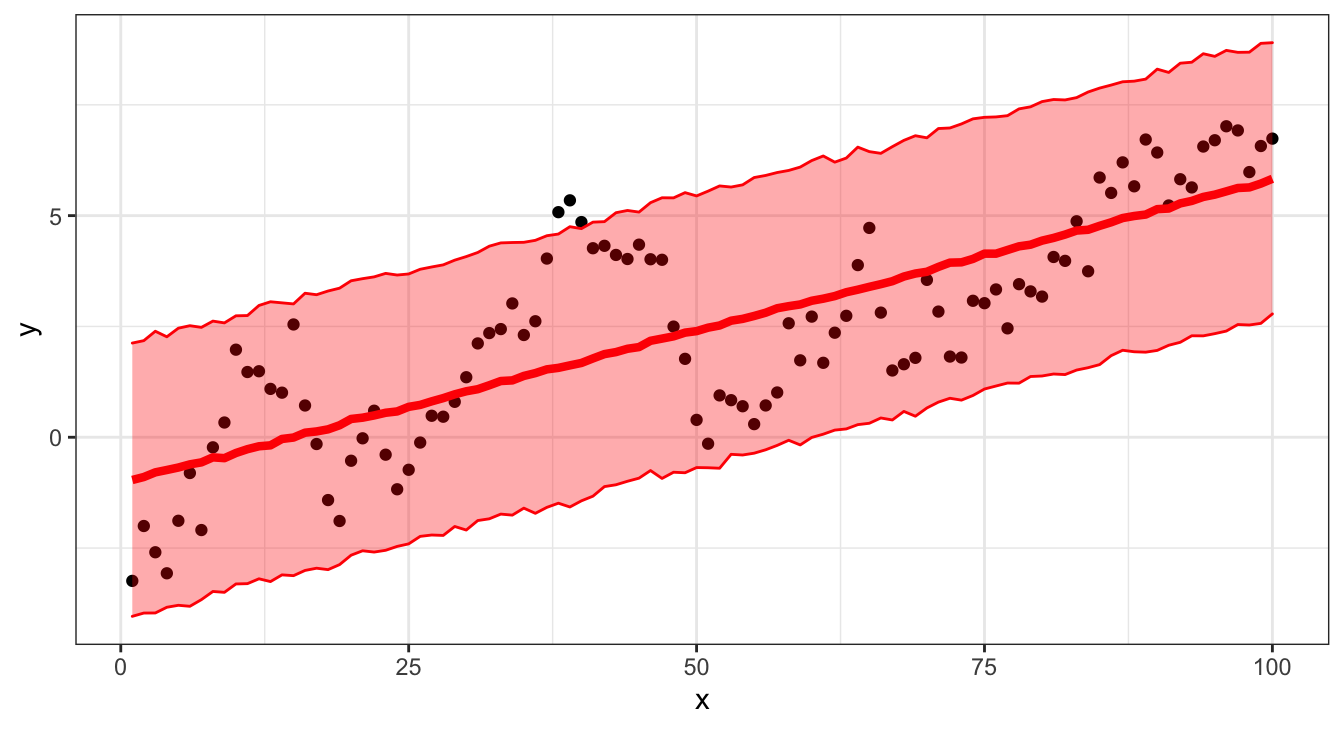
\includegraphics[width=\textwidth]{Lec20_files/figure-beamer/unnamed-chunk-16-1} \end{center}

\end{frame}

\begin{frame}[fragile,t]{\texttt{spBayes} GLM Model}
\protect\hypertarget{spbayes-glm-model}{}

\footnoteoutput

\begin{Shaded}
\begin{Highlighting}[]
\NormalTok{spg =}\StringTok{ }\NormalTok{spBayes}\OperatorTok{::}\KeywordTok{spGLM}\NormalTok{(}
\NormalTok{  no_inf}\OperatorTok{/}\NormalTok{no_exam }\OperatorTok{~}\StringTok{ }\NormalTok{elev}\OperatorTok{:}\NormalTok{elev_f }\OperatorTok{+}\StringTok{ }\NormalTok{max9901}\OperatorTok{:}\NormalTok{max_f }\OperatorTok{+}\StringTok{ }\NormalTok{stdev9901, }
  
  \DataTypeTok{data=}\NormalTok{loaloa, }\DataTypeTok{family=}\StringTok{"binomial"}\NormalTok{, }\DataTypeTok{weights=}\NormalTok{loaloa}\OperatorTok{$}\NormalTok{no_exam, }
  
  \DataTypeTok{coords=}\KeywordTok{cbind}\NormalTok{(loaloa}\OperatorTok{$}\NormalTok{longitude, loaloa}\OperatorTok{$}\NormalTok{latitude),}
  
  \DataTypeTok{cov.model=}\StringTok{"exponential"}\NormalTok{, }\DataTypeTok{n.samples=}\DecValTok{20000}\NormalTok{,}
  
  \DataTypeTok{starting=}\KeywordTok{list}\NormalTok{(}\DataTypeTok{beta=}\KeywordTok{rep}\NormalTok{(}\DecValTok{0}\NormalTok{,}\DecValTok{7}\NormalTok{), }\DataTypeTok{phi=}\DecValTok{3}\NormalTok{, }\DataTypeTok{sigma.sq=}\DecValTok{1}\NormalTok{, }\DataTypeTok{w=}\DecValTok{0}\NormalTok{),}
  
  \DataTypeTok{priors=}\KeywordTok{list}\NormalTok{(}\DataTypeTok{phi.unif=}\KeywordTok{c}\NormalTok{(}\FloatTok{0.1}\NormalTok{, }\DecValTok{10}\NormalTok{), }\DataTypeTok{sigma.sq.ig=}\KeywordTok{c}\NormalTok{(}\DecValTok{2}\NormalTok{, }\DecValTok{2}\NormalTok{)),}
  
  \DataTypeTok{amcmc=}\KeywordTok{list}\NormalTok{(}\DataTypeTok{n.batch=}\DecValTok{1000}\NormalTok{, }\DataTypeTok{batch.length=}\DecValTok{20}\NormalTok{, }\DataTypeTok{accept.rate=}\FloatTok{0.43}\NormalTok{))}

\KeywordTok{save}\NormalTok{(spg, loaloa, }\DataTypeTok{file=}\StringTok{"loaloa.Rdata"}\NormalTok{)}
\end{Highlighting}
\end{Shaded}

\end{frame}

\begin{frame}[fragile]{}
\protect\hypertarget{section}{}

\footnotesize

\begin{Shaded}
\begin{Highlighting}[]
\NormalTok{spg}\OperatorTok{$}\NormalTok{p.beta.theta.samples }\OperatorTok\StringTok{ }
\StringTok{  }\KeywordTok{post_summary}\NormalTok{() }\OperatorTok\StringTok{ }
\StringTok{  }\NormalTok{knitr}\OperatorTok{::}\KeywordTok{kable}\NormalTok{(}\DataTypeTok{digits=}\DecValTok{5}\NormalTok{)}
\end{Highlighting}
\end{Shaded}

\begin{longtable}[]{@{}lrrrr@{}}
\toprule
param & post\_mean & post\_med & post\_lower &
post\_upper\tabularnewline
\midrule
\endhead
(Intercept) & -7.62467 & -7.10607 & -15.33201 & -1.56786\tabularnewline
stdev9901 & 1.77896 & -0.26705 & -19.15846 & 24.59887\tabularnewline
elev:elev\_f(0,1000{]} & 0.00010 & 0.00065 & -0.00780 &
0.00316\tabularnewline
elev:elev\_f(1000,1300{]} & -0.00059 & -0.00035 & -0.00471 &
0.00176\tabularnewline
elev:elev\_f(1300,2000{]} & -0.01448 & -0.01064 & -0.04942 &
-0.00030\tabularnewline
max9901:max\_f(0,0.8{]} & 0.08517 & -0.78200 & -6.96111 &
9.06059\tabularnewline
max9901:max\_f(0.8,1{]} & 0.69926 & -0.25813 & -5.79400 &
9.08833\tabularnewline
sigma.sq & 0.45277 & 0.39071 & 0.14322 & 1.17856\tabularnewline
phi & 2.12385 & 1.44856 & 0.12026 & 8.46872\tabularnewline
\bottomrule
\end{longtable}

\end{frame}

\begin{frame}{Prediction}
\protect\hypertarget{prediction}{}

\begin{center}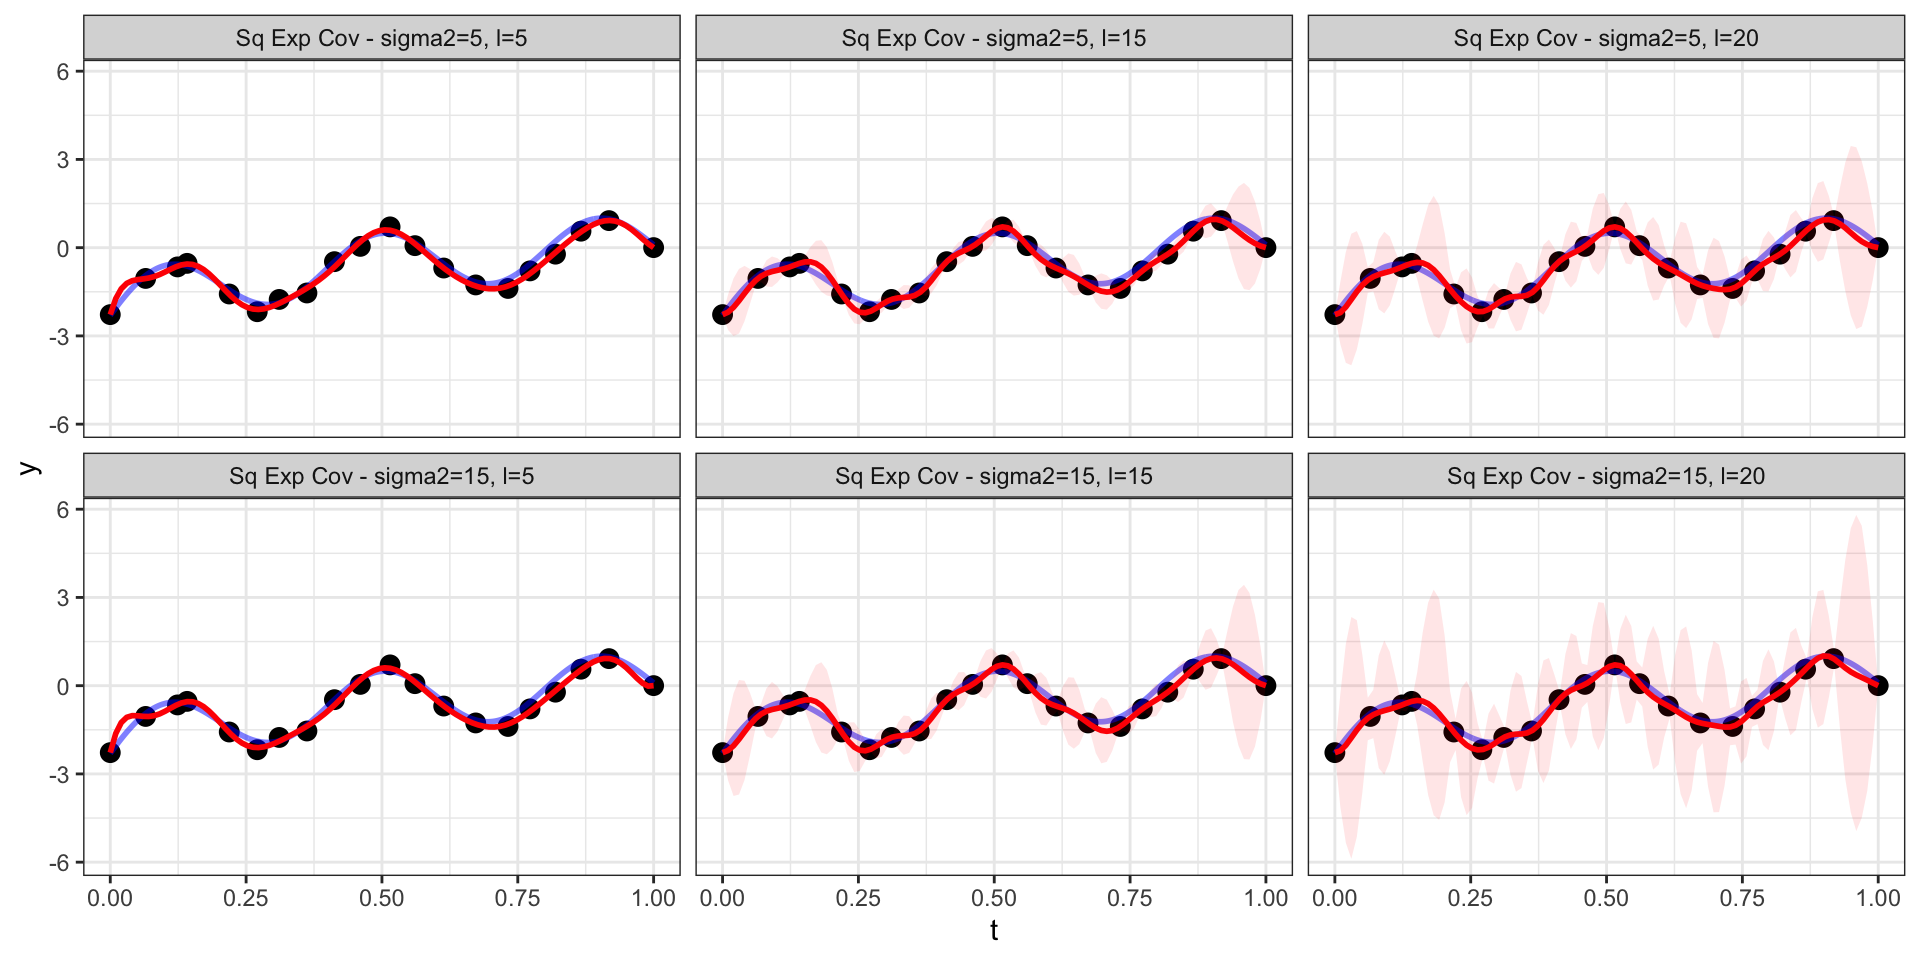
\includegraphics[width=\textwidth]{Lec20_files/figure-beamer/unnamed-chunk-20-1} \end{center}

\end{frame}

\begin{frame}[fragile,t]{\texttt{spBayes} GLM Model - Fixed?}
\protect\hypertarget{spbayes-glm-model---fixed}{}

\begin{Shaded}
\begin{Highlighting}[]
\NormalTok{spg_fix =}\StringTok{ }\NormalTok{spBayes}\OperatorTok{::}\KeywordTok{spGLM}\NormalTok{(}
\NormalTok{  no_inf }\OperatorTok{~}\StringTok{ }\NormalTok{elev}\OperatorTok{:}\NormalTok{elev_f }\OperatorTok{+}\StringTok{ }\NormalTok{max9901}\OperatorTok{:}\NormalTok{max_f }\OperatorTok{+}\StringTok{ }\NormalTok{stdev9901, }
  
  \DataTypeTok{data=}\NormalTok{loaloa, }\DataTypeTok{family=}\StringTok{"binomial"}\NormalTok{, }\DataTypeTok{weights=}\NormalTok{loaloa}\OperatorTok{$}\NormalTok{no_exam, }
  
  \DataTypeTok{coords=}\KeywordTok{cbind}\NormalTok{(loaloa}\OperatorTok{$}\NormalTok{longitude, loaloa}\OperatorTok{$}\NormalTok{latitude),}
  
  \DataTypeTok{cov.model=}\StringTok{"exponential"}\NormalTok{, }\DataTypeTok{n.samples=}\DecValTok{20000}\NormalTok{,}
  
  \DataTypeTok{starting=}\KeywordTok{list}\NormalTok{(}\DataTypeTok{beta=}\KeywordTok{rep}\NormalTok{(}\DecValTok{0}\NormalTok{,}\DecValTok{7}\NormalTok{), }\DataTypeTok{phi=}\DecValTok{3}\NormalTok{, }\DataTypeTok{sigma.sq=}\DecValTok{1}\NormalTok{, }\DataTypeTok{w=}\DecValTok{0}\NormalTok{),}
  
  \DataTypeTok{priors=}\KeywordTok{list}\NormalTok{(}\DataTypeTok{phi.unif=}\KeywordTok{c}\NormalTok{(}\FloatTok{0.1}\NormalTok{, }\DecValTok{10}\NormalTok{), }\DataTypeTok{sigma.sq.ig=}\KeywordTok{c}\NormalTok{(}\DecValTok{2}\NormalTok{, }\DecValTok{2}\NormalTok{)),}
  
  \DataTypeTok{amcmc=}\KeywordTok{list}\NormalTok{(}\DataTypeTok{n.batch=}\DecValTok{1000}\NormalTok{, }\DataTypeTok{batch.length=}\DecValTok{20}\NormalTok{, }\DataTypeTok{accept.rate=}\FloatTok{0.43}\NormalTok{)}
\NormalTok{)}

\KeywordTok{save}\NormalTok{(spg_fix, loaloa, }\DataTypeTok{file=}\StringTok{"loaloa_fix.Rdata"}\NormalTok{)}
\end{Highlighting}
\end{Shaded}

\end{frame}

\begin{frame}{}
\protect\hypertarget{section-1}{}

\footnotesize

\begin{longtable}[]{@{}lrrrr@{}}
\toprule
param & post\_mean & post\_med & post\_lower &
post\_upper\tabularnewline
\midrule
\endhead
(Intercept) & -3.14223 & -3.43877 & -4.38140 & -1.01108\tabularnewline
stdev9901 & 1.88811 & 1.02957 & -5.28818 & 9.04674\tabularnewline
elev:elev\_f(0,1000{]} & 0.00036 & 0.00048 & -0.00069 &
0.00114\tabularnewline
elev:elev\_f(1000,1300{]} & -0.00036 & -0.00031 & -0.00127 &
0.00039\tabularnewline
elev:elev\_f(1300,2000{]} & -0.00209 & -0.00206 & -0.00310 &
-0.00131\tabularnewline
max9901:max\_f(0,0.8{]} & 0.74129 & 0.55728 & -0.98971 &
2.78417\tabularnewline
max9901:max\_f(0.8,1{]} & 1.15469 & 0.92740 & -0.18829 &
2.89406\tabularnewline
sigma.sq & 1.26052 & 1.21204 & 0.32891 & 2.36502\tabularnewline
phi & 2.51439 & 2.38441 & 1.08064 & 4.86766\tabularnewline
\bottomrule
\end{longtable}

\end{frame}

\begin{frame}{Fit - Training}
\protect\hypertarget{fit---training-1}{}

\begin{center}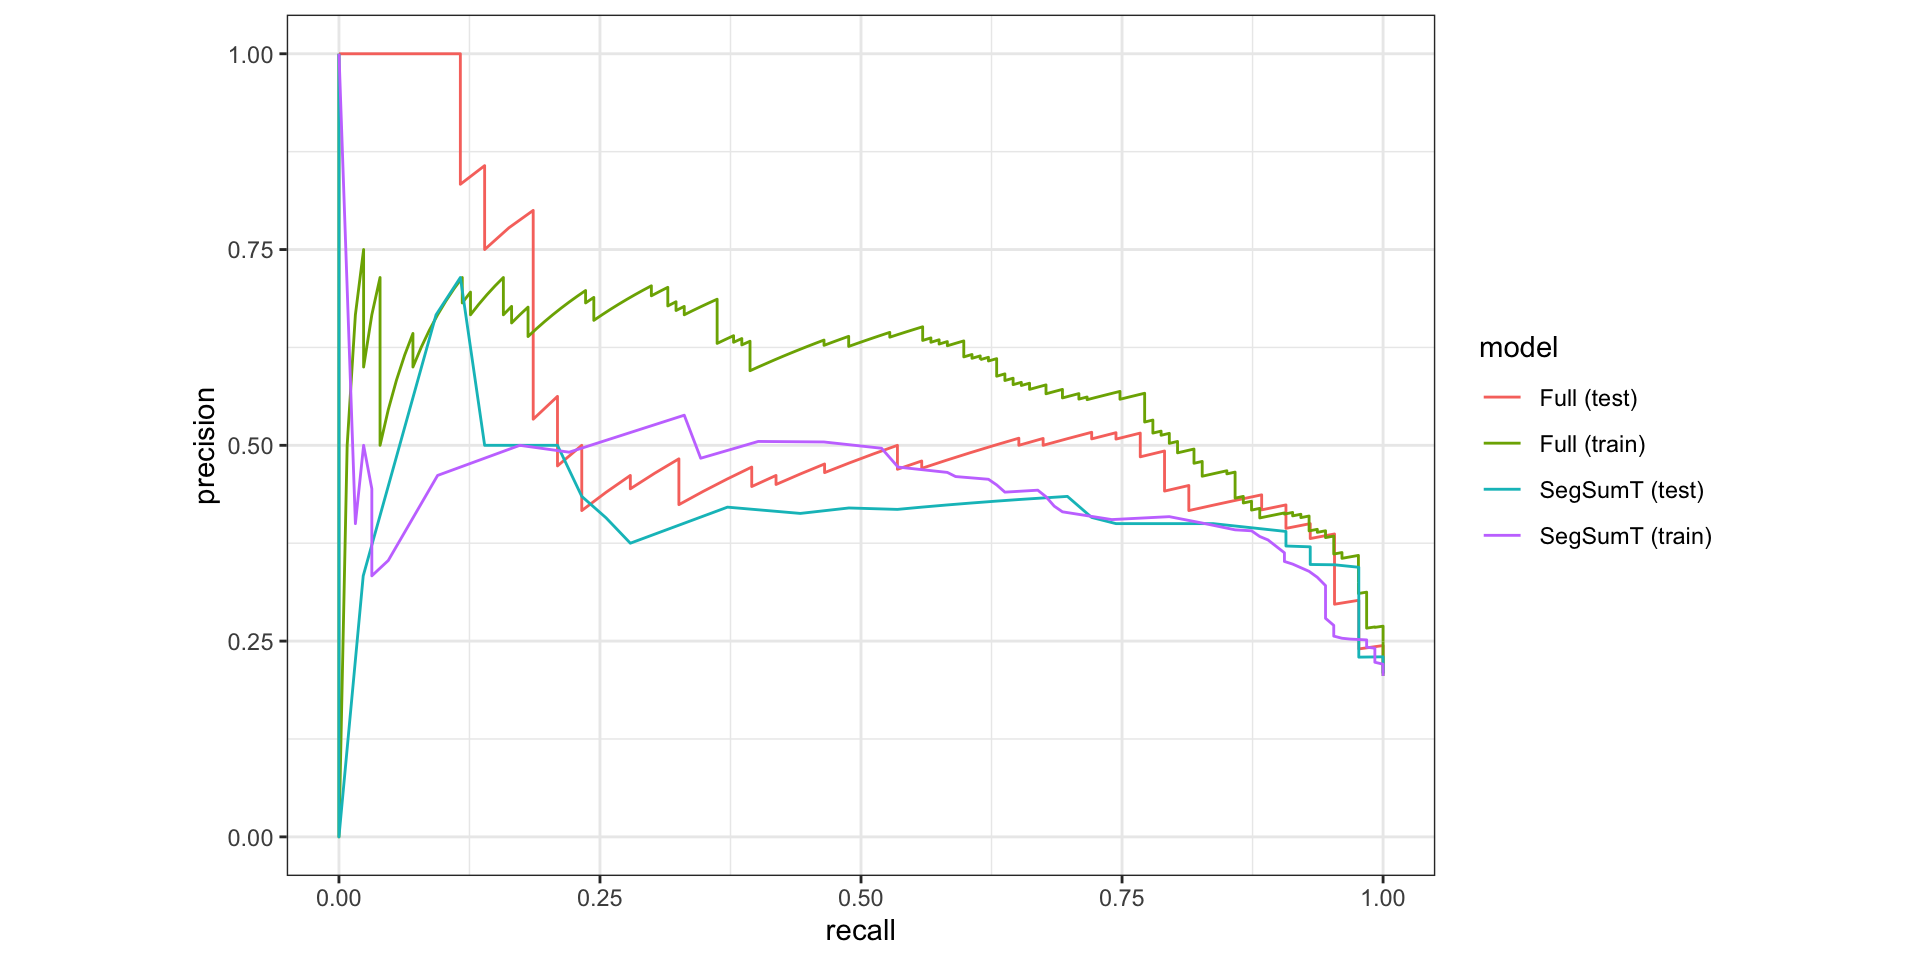
\includegraphics[width=\textwidth]{Lec20_files/figure-beamer/unnamed-chunk-24-1} \end{center}

\end{frame}

\begin{frame}{Fit - Testing}
\protect\hypertarget{fit---testing-1}{}

\begin{center}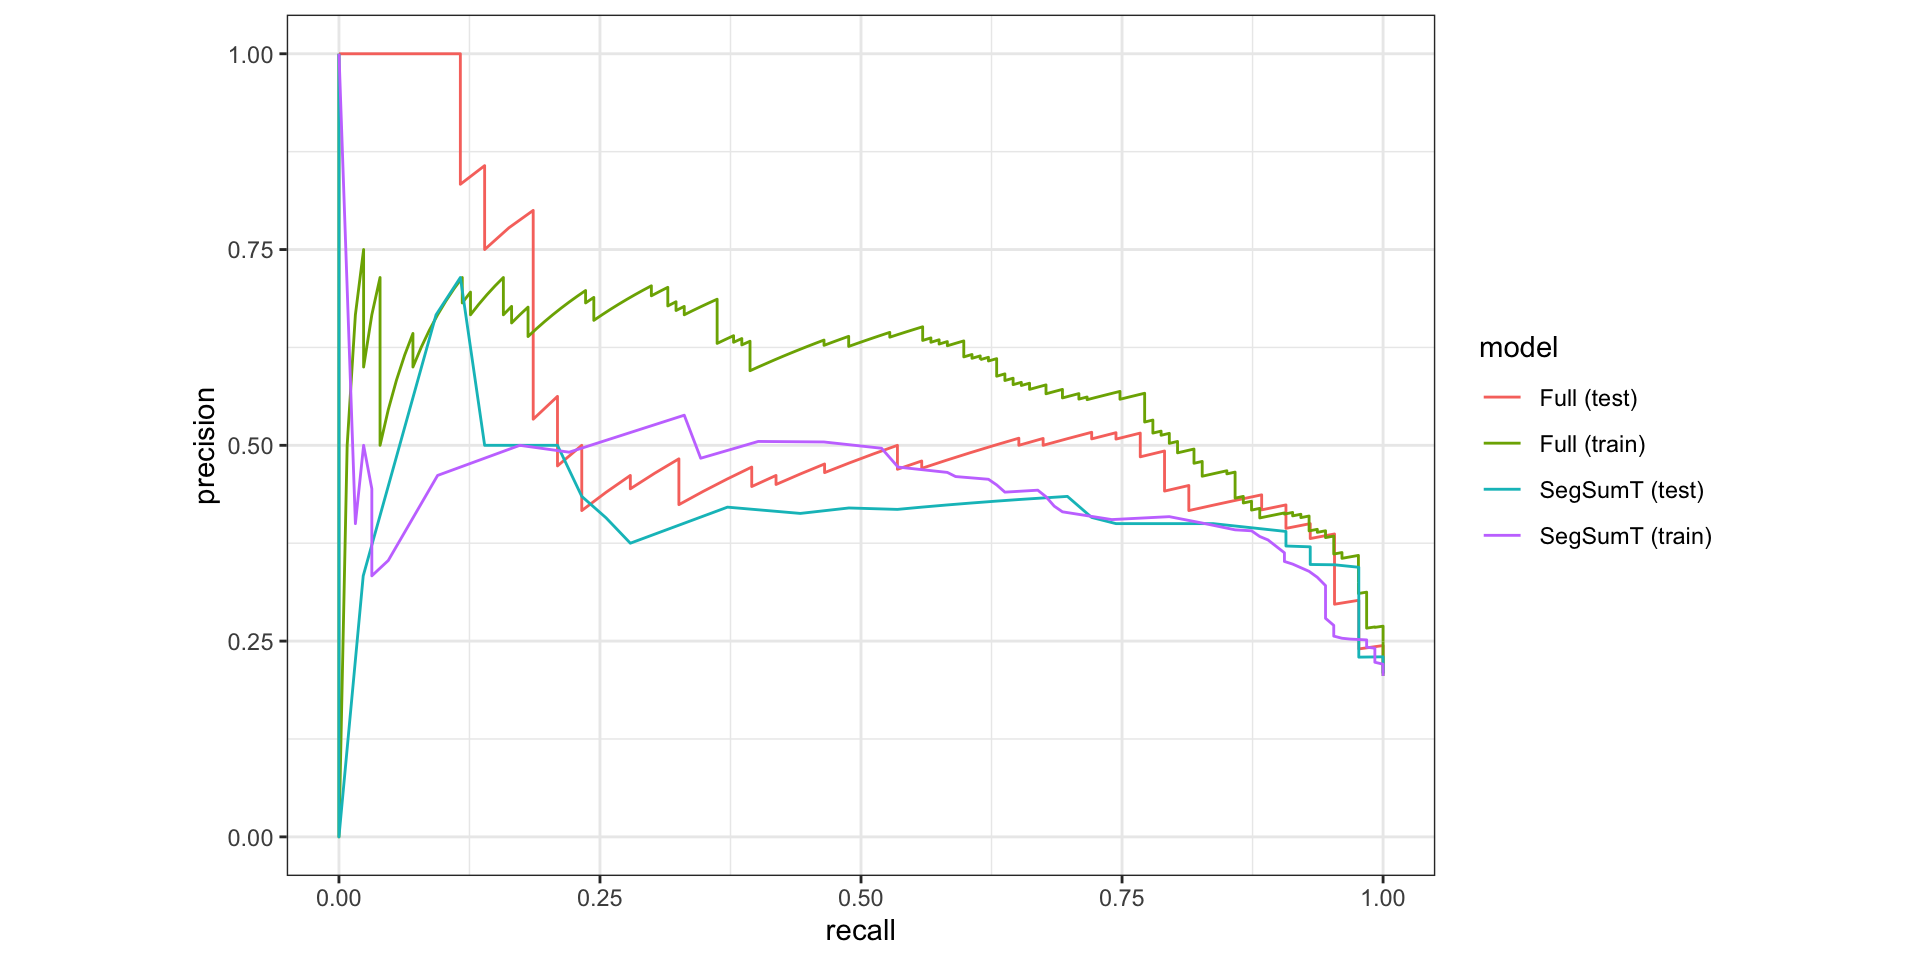
\includegraphics[width=\textwidth]{Lec20_files/figure-beamer/unnamed-chunk-25-1} \end{center}

\end{frame}

\begin{frame}{Diggle's Predictive Surface}
\protect\hypertarget{diggles-predictive-surface}{}

\begin{center}
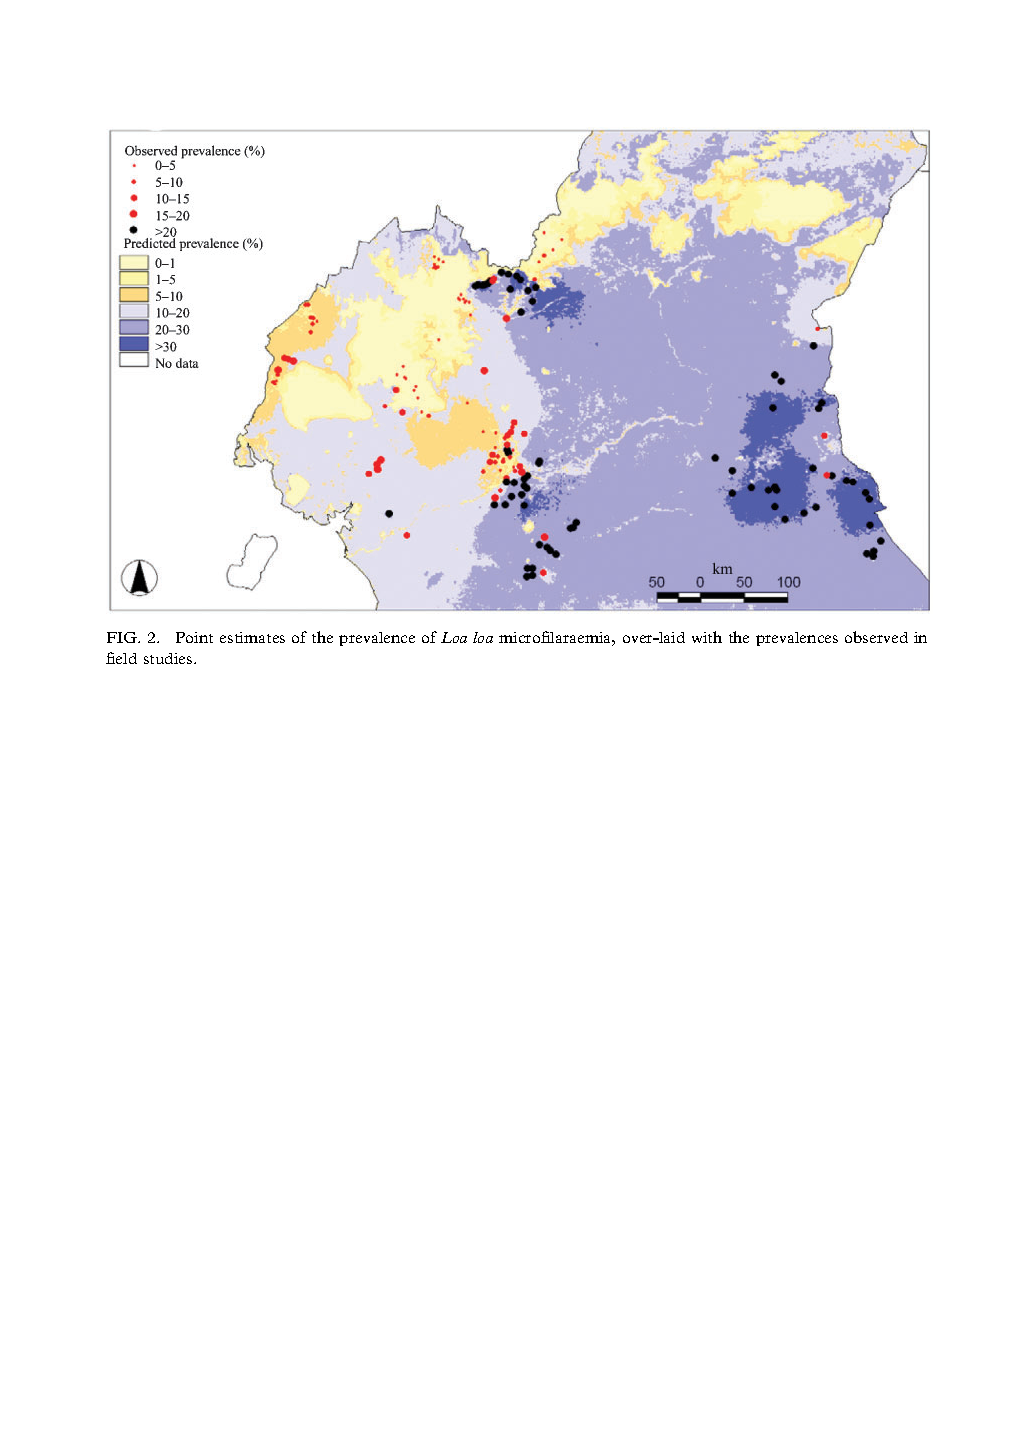
\includegraphics[width=0.9\textwidth]{figs/diggle_fig2.pdf}
\end{center}

\end{frame}

\begin{frame}{Exceedance Probability - Posterior Summary}
\protect\hypertarget{exceedance-probability---posterior-summary}{}

\begin{center}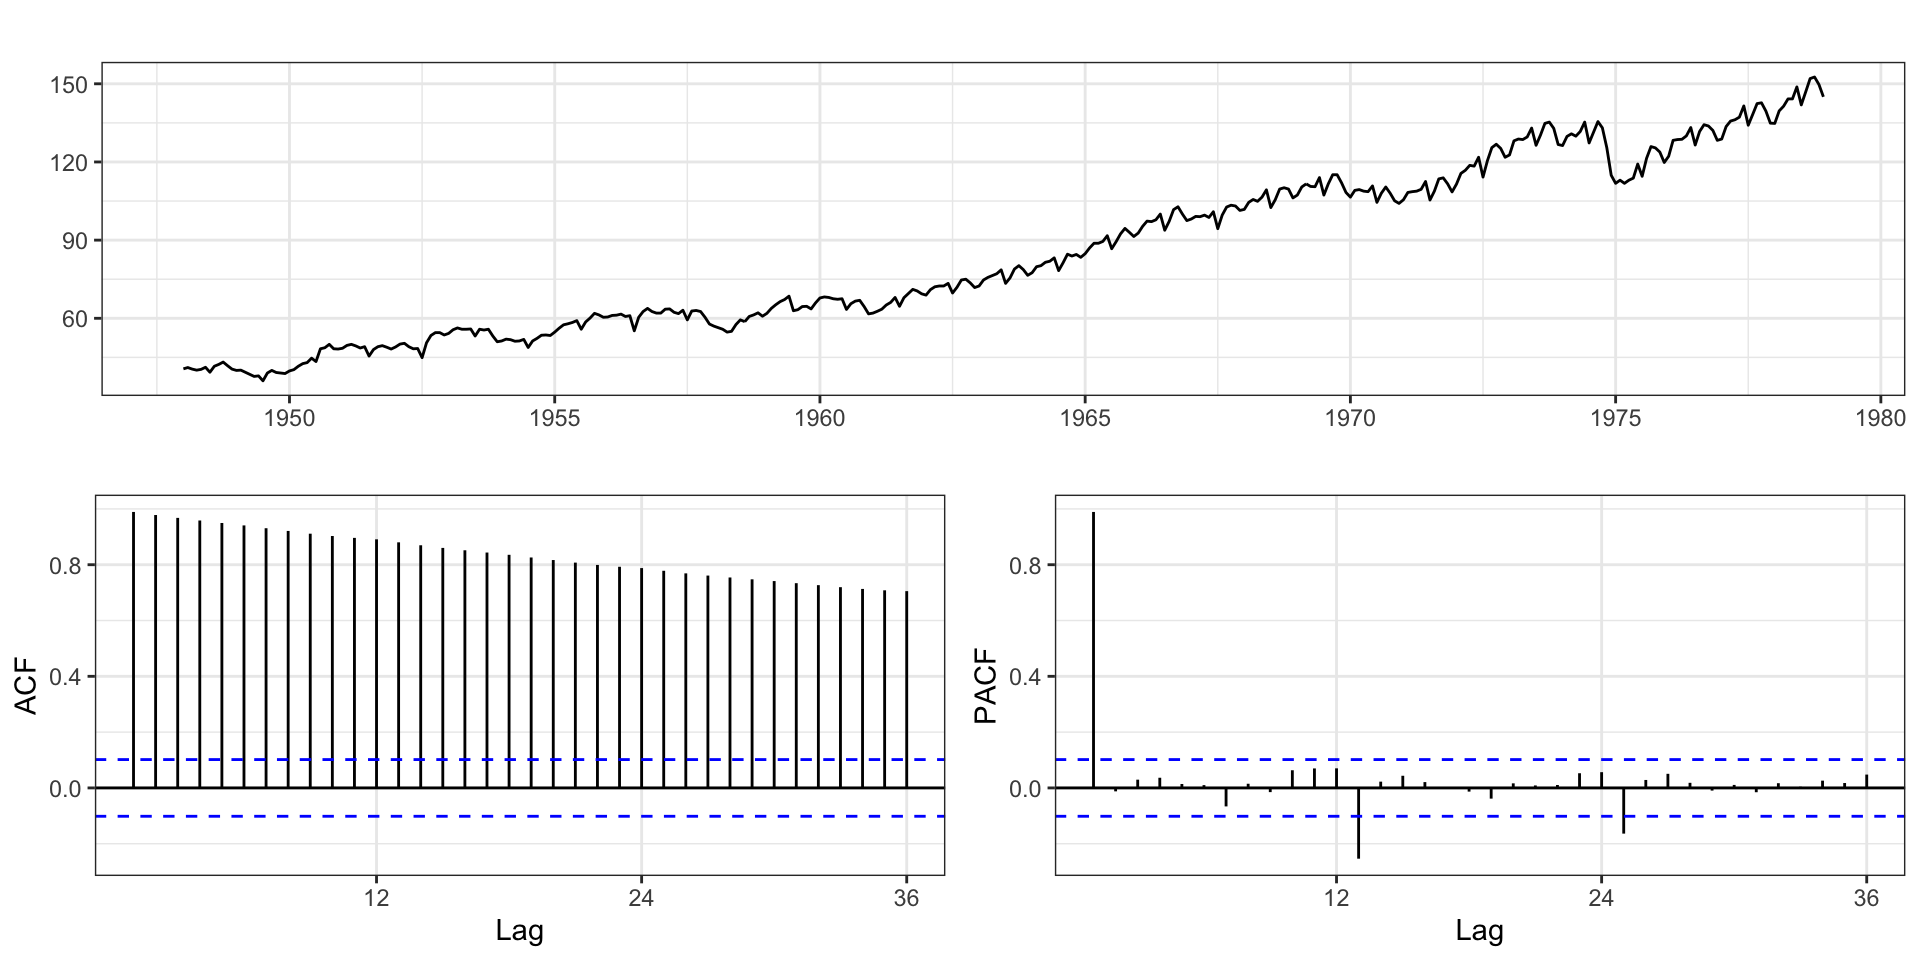
\includegraphics[width=\textwidth]{Lec20_files/figure-beamer/unnamed-chunk-26-1} \end{center}

\end{frame}

\begin{frame}{Exceedance Probability Predictive Surface}
\protect\hypertarget{exceedance-probability-predictive-surface}{}

\begin{center}
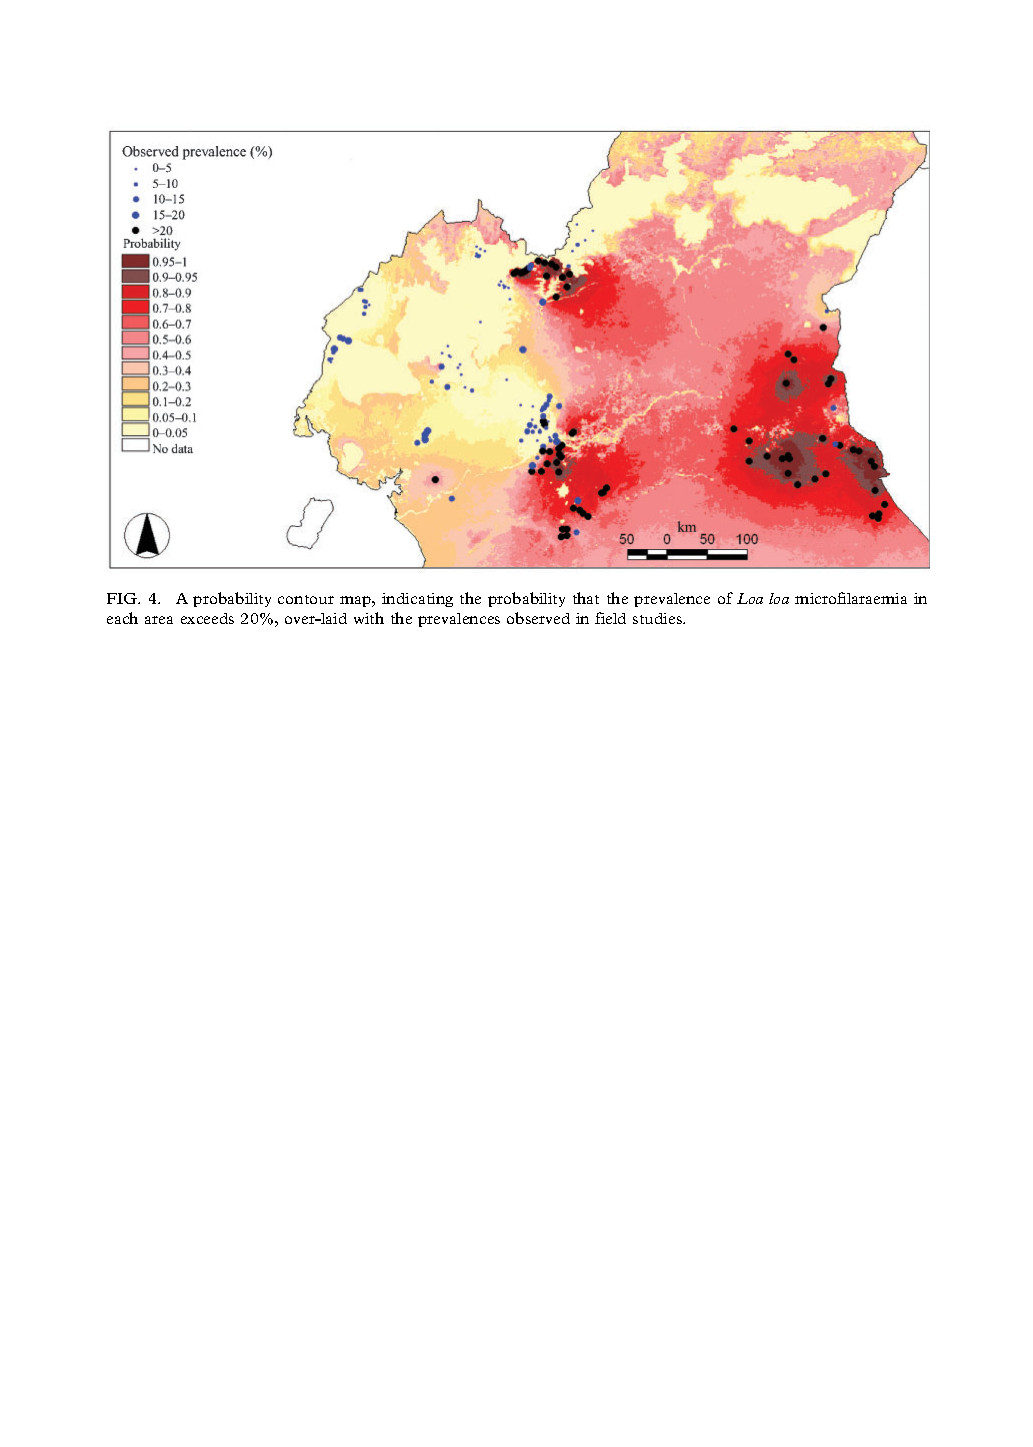
\includegraphics[width=0.9\textwidth]{figs/diggle_fig4.pdf}
\end{center}

\end{frame}

\hypertarget{spatial-assignment-of-migratory-birds}{%
\section{Spatial Assignment of Migratory
Birds}\label{spatial-assignment-of-migratory-birds}}

\begin{frame}{Background}
\protect\hypertarget{background}{}

Using intrinsic markers (genetic and isotopic signals) for the purpose
of inferring migratory connectivity.

\vspace{2mm}

\begin{itemize}
\tightlist
\item
  Existing methods are too coarse for most applications
\end{itemize}

\vspace{2mm}

\begin{itemize}
\tightlist
\item
  Large amounts of data are available ( \textgreater 150,000 feather
  samples from \textgreater 500 species)
\end{itemize}

\vspace{2mm}

\begin{itemize}
\tightlist
\item
  Genetic assignment methods are based on Wasser, et al.~(2004)
\end{itemize}

\vspace{2mm}

\begin{itemize}
\tightlist
\item
  Isotopic assignment methods are based on Wunder, et al.~(2005)
\end{itemize}

\end{frame}

\begin{frame}{Data - DNA microsatellites and \(\delta \isotope[2]{H}\)}
\protect\hypertarget{data---dna-microsatellites-and-delta-isotope2h}{}

\begin{columns}[t]
\column{0.5\textwidth}
Hermit Thrush (\textit{Catharus guttatus}) \\
\vspace{2mm}
\begin{itemize}
\item 138 individuals
\item 14 locations
\item 6 loci
\item 9-27 alleles / locus
\end{itemize}
\column{0.5\textwidth}
Wilson's Warbler (\textit{Wilsonia pusilla}) \\
\vspace{2mm}
\begin{itemize}
\item 163 individuals
\item 8 locations
\item 9 loci
\item 15-31 alleles / locus
\end{itemize}

\end{columns}

\vspace{5mm}

\begin{columns}[t]
\column{0.5\textwidth}
\begin{center}
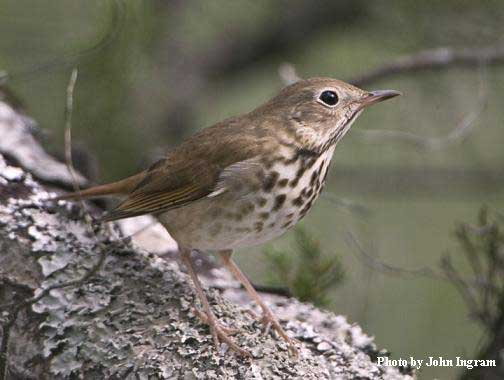
\includegraphics[width=0.65\textwidth]{figs/hermit_thrush.jpeg}
\end{center}
\column{0.5\textwidth}
\begin{center}
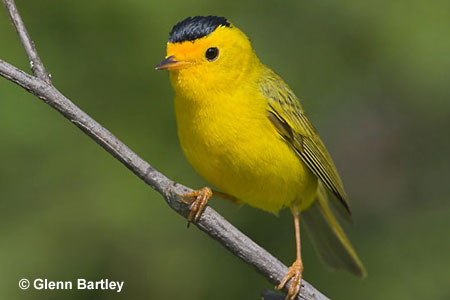
\includegraphics[width=0.65\textwidth]{figs/wilsons_warbler.jpeg}
\end{center}
\end{columns}

\end{frame}

\begin{frame}{Sampling Locations}
\protect\hypertarget{sampling-locations}{}

\begin{center}
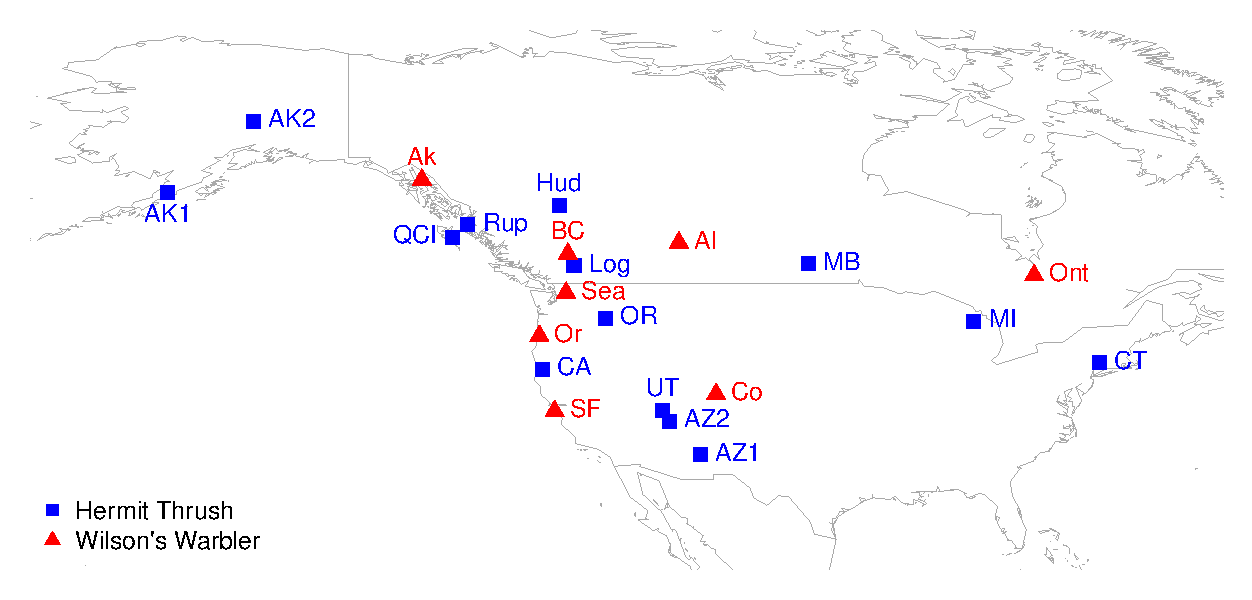
\includegraphics[width=\textwidth]{figs/sampling_locs.pdf}
\end{center}

\end{frame}

\begin{frame}{Allele Frequency Model}
\protect\hypertarget{allele-frequency-model}{}

For the allele \(i\), from locus \(l\), at location \(k\)

\[
\begin{aligned}
\symbf{y}_{\cdot l k}|\symbf{\Theta} &\sim \mathcal{N}\left(\textstyle\sum_i y_{ilk},\: \symbf{f}_{\cdot l k}\right) \\
\\
f_{ilk} &= \frac{\exp(\Theta_{ilk})}{\sum_i \exp(\Theta_{ilk})} \\
\\
\symbf{\Theta}_{il}|\symbf{\alpha},\symbf{\mu} &\sim \mathcal{N}( \symbf{\mu}_{il},\, \symbf{\Sigma_{}}) \\
\end{aligned}
\]

\[ \left\{\Sigma\right\}_{ij} = \sigma^2 \, \exp \Big(-(\{d\}_{ij}\, r)^{\psi} \Big) + \sigma^2_n \, {1}_{i=j} \]

\end{frame}

\begin{frame}{Predictions by Allele (Locus 3)}
\protect\hypertarget{predictions-by-allele-locus-3}{}

\begin{center}
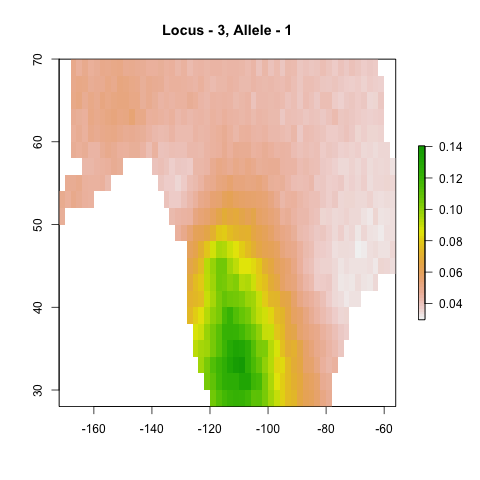
\includegraphics[width=0.25\textwidth]{figs/allele3/Med-Al3-1.png}
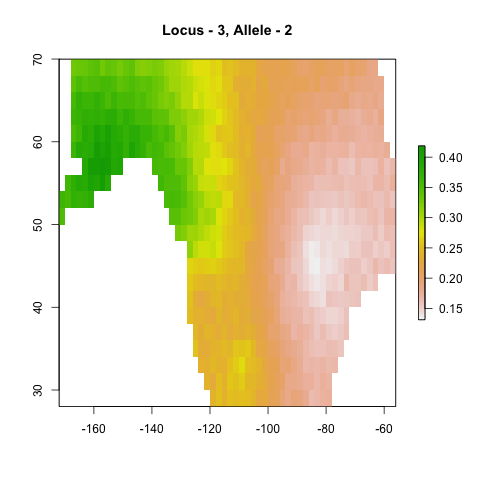
\includegraphics[width=0.25\textwidth]{figs/allele3/Med-Al3-2.png}
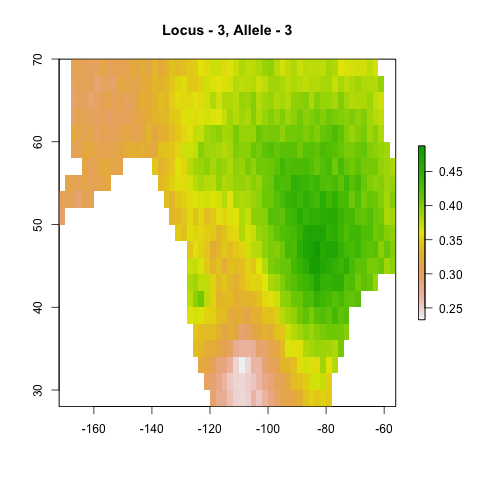
\includegraphics[width=0.25\textwidth]{figs/allele3/Med-Al3-3.png} \\
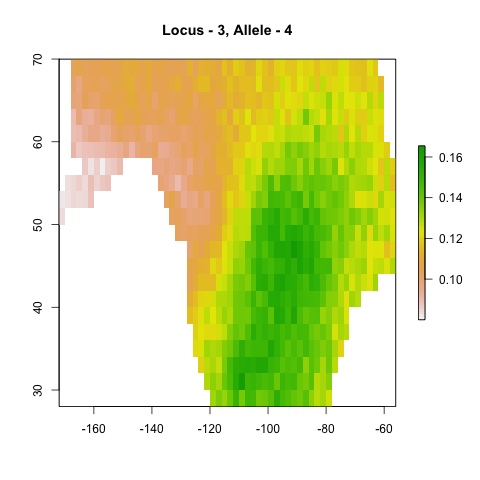
\includegraphics[width=0.25\textwidth]{figs/allele3/Med-Al3-4.png}
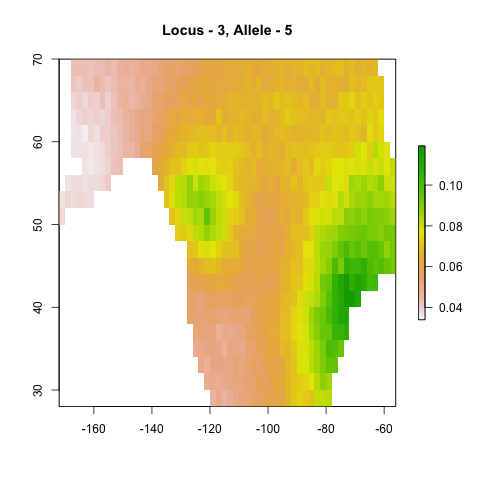
\includegraphics[width=0.25\textwidth]{figs/allele3/Med-Al3-5.png}
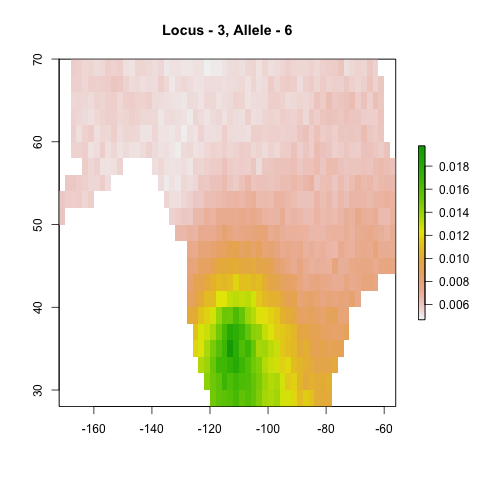
\includegraphics[width=0.25\textwidth]{figs/allele3/Med-Al3-6.png} \\
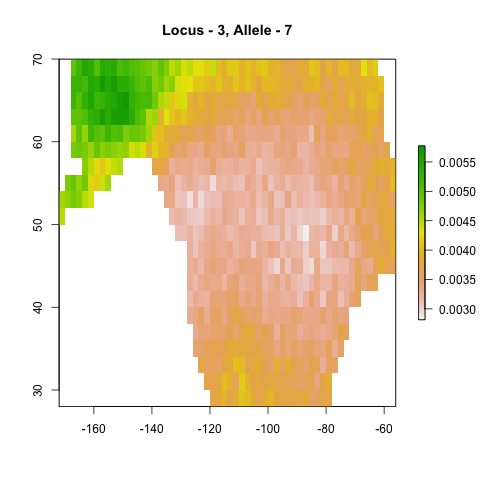
\includegraphics[width=0.25\textwidth]{figs/allele3/Med-Al3-7.png}
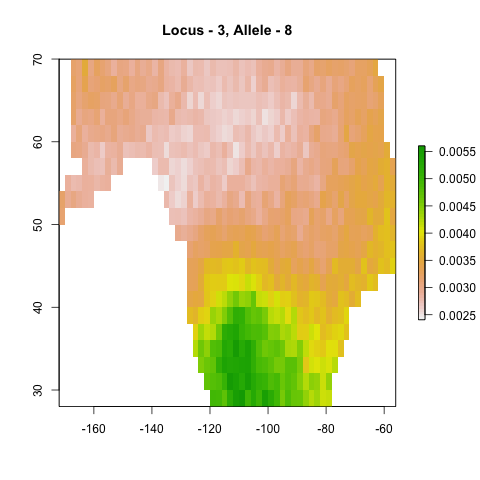
\includegraphics[width=0.25\textwidth]{figs/allele3/Med-Al3-8.png}
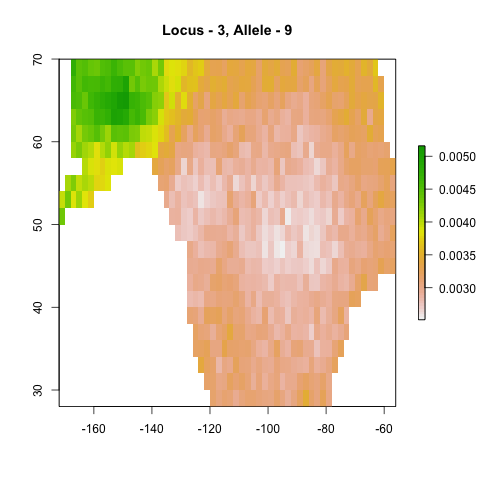
\includegraphics[width=0.25\textwidth]{figs/allele3/Med-Al3-9.png}
\end{center}

\end{frame}

\begin{frame}{Genetic Assignment Model}
\protect\hypertarget{genetic-assignment-model}{}

Assignment model assuming Hardy-Weinberg equilibrium and allowing for
genotyping (\(\delta\)) and single amplification (\(\gamma\)) errors.

\[
\begin{aligned}
P(S_G|\symbf{f},k) &= \prod_l P(i_l, j_l | \symbf{f},k) \\
\\
P(i_l, j_l | \symbf{f},k) &= 
\begin{cases}
\gamma P(i_l|\symbf{f},k) + (1-\gamma)P(i_l|\symbf{\tilde f},k)^2 & \text{if $i=j$} \vspace{2mm} \\
(1-\gamma) P(i_l|\symbf{f},k) P(j_l|\symbf{f},k)      & \text{if $i \ne j$}
\end{cases} \\
\\
P(i_l|\symbf{f},k) &= (1-\delta) f_{lik} + \delta / m_l
\end{aligned}
\]

\end{frame}

\begin{frame}{Combined Model}
\protect\hypertarget{combined-model}{}

\begin{center}
Genetic \qquad\qquad\qquad\quad
Isotopic \qquad\qquad\qquad\quad
Combined
\end{center}

\begin{center}
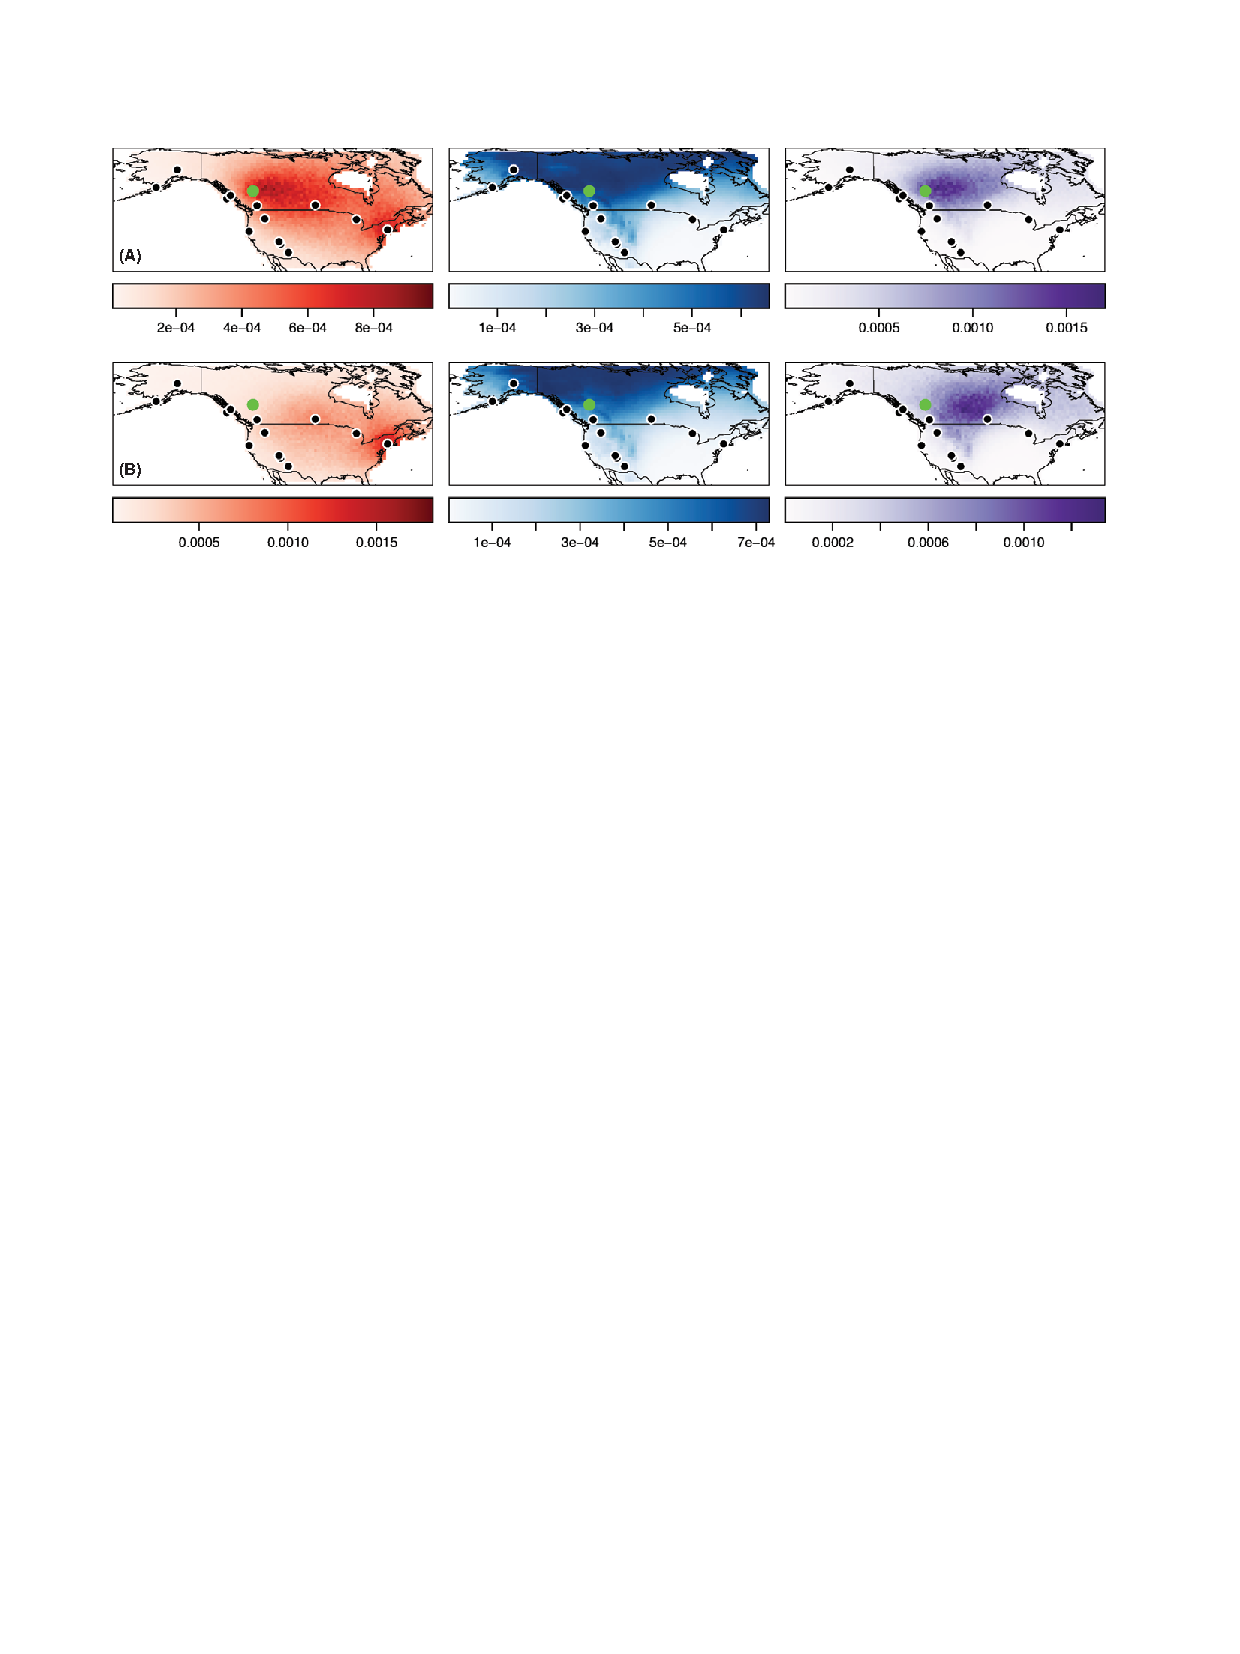
\includegraphics[width=\textwidth]{figs/hermit_maps.pdf}
\end{center}

\end{frame}

\begin{frame}{Model Assessment}
\protect\hypertarget{model-assessment}{}

\begin{center}
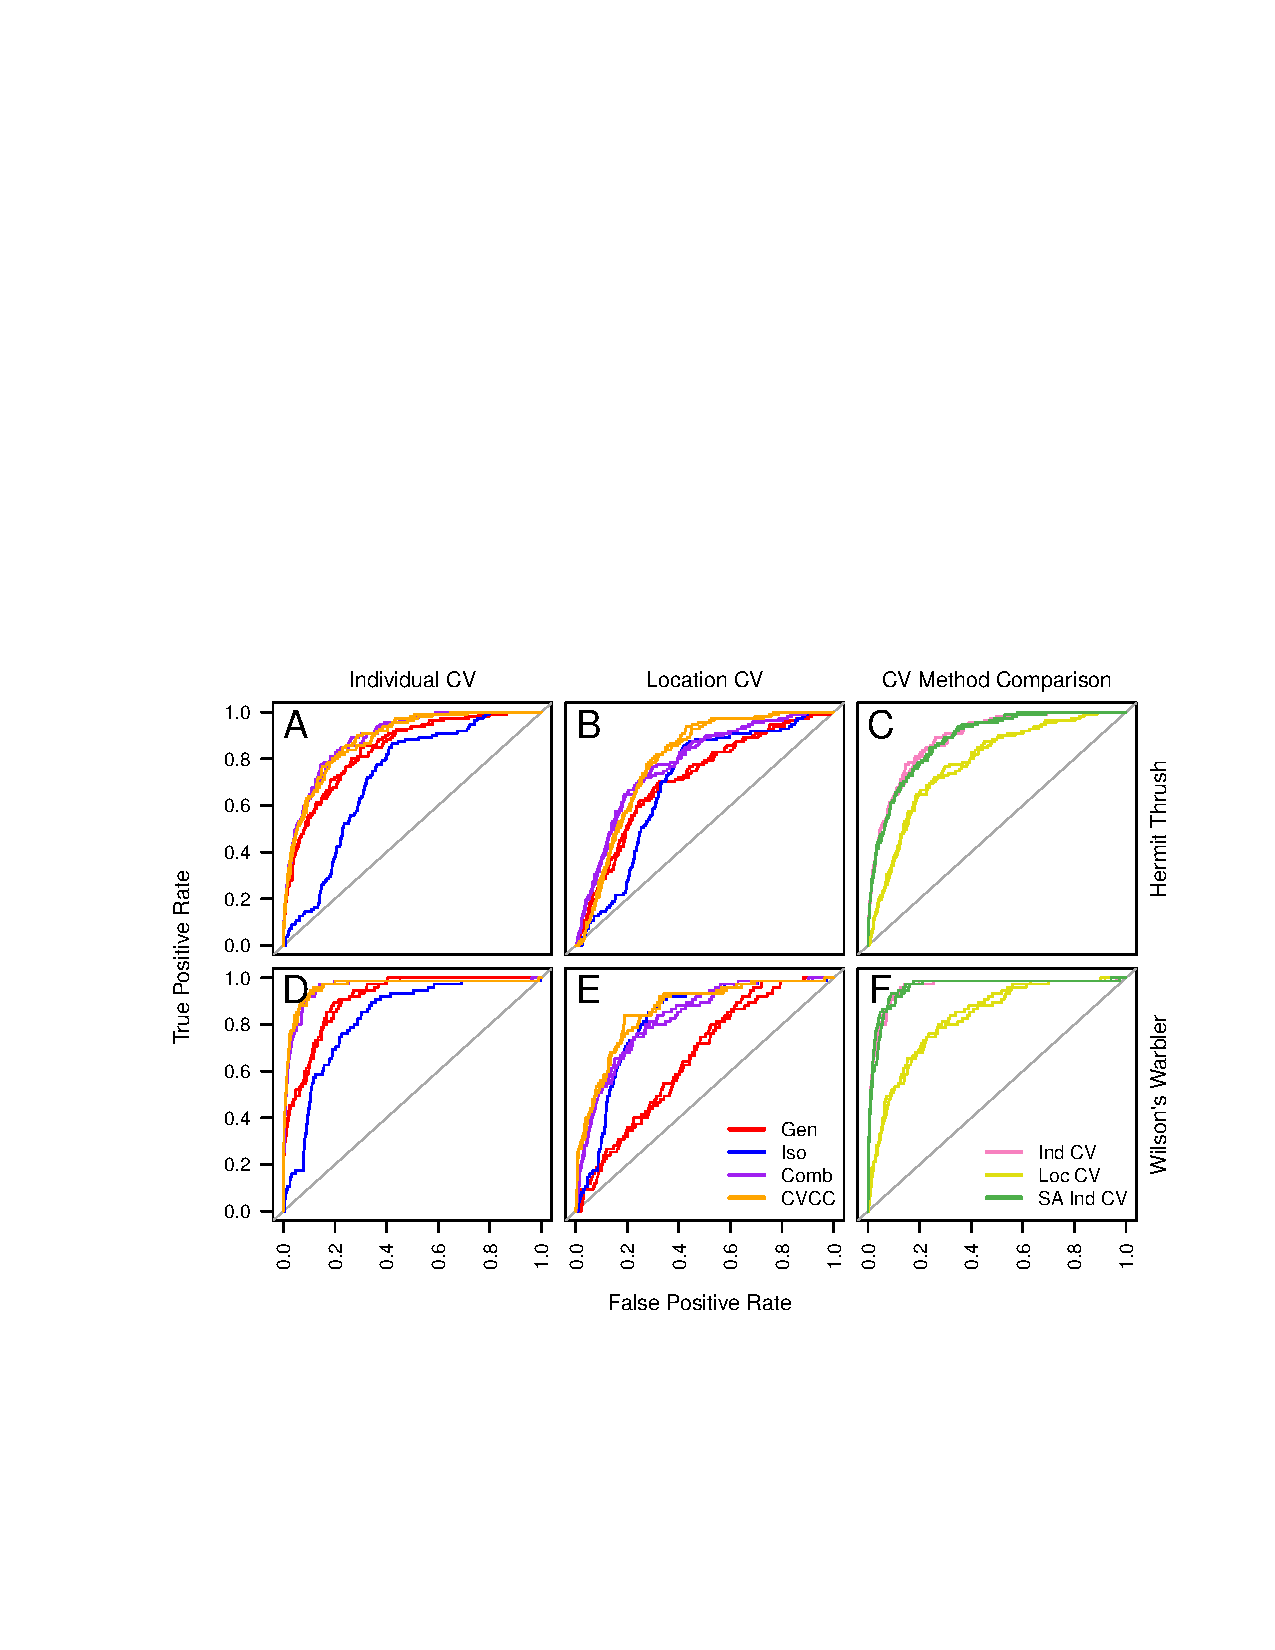
\includegraphics[width=\textwidth]{figs/ROCs.pdf}
\end{center}

\end{frame}

\begin{frame}{Migratory Connectivity}
\protect\hypertarget{migratory-connectivity}{}

\begin{center}
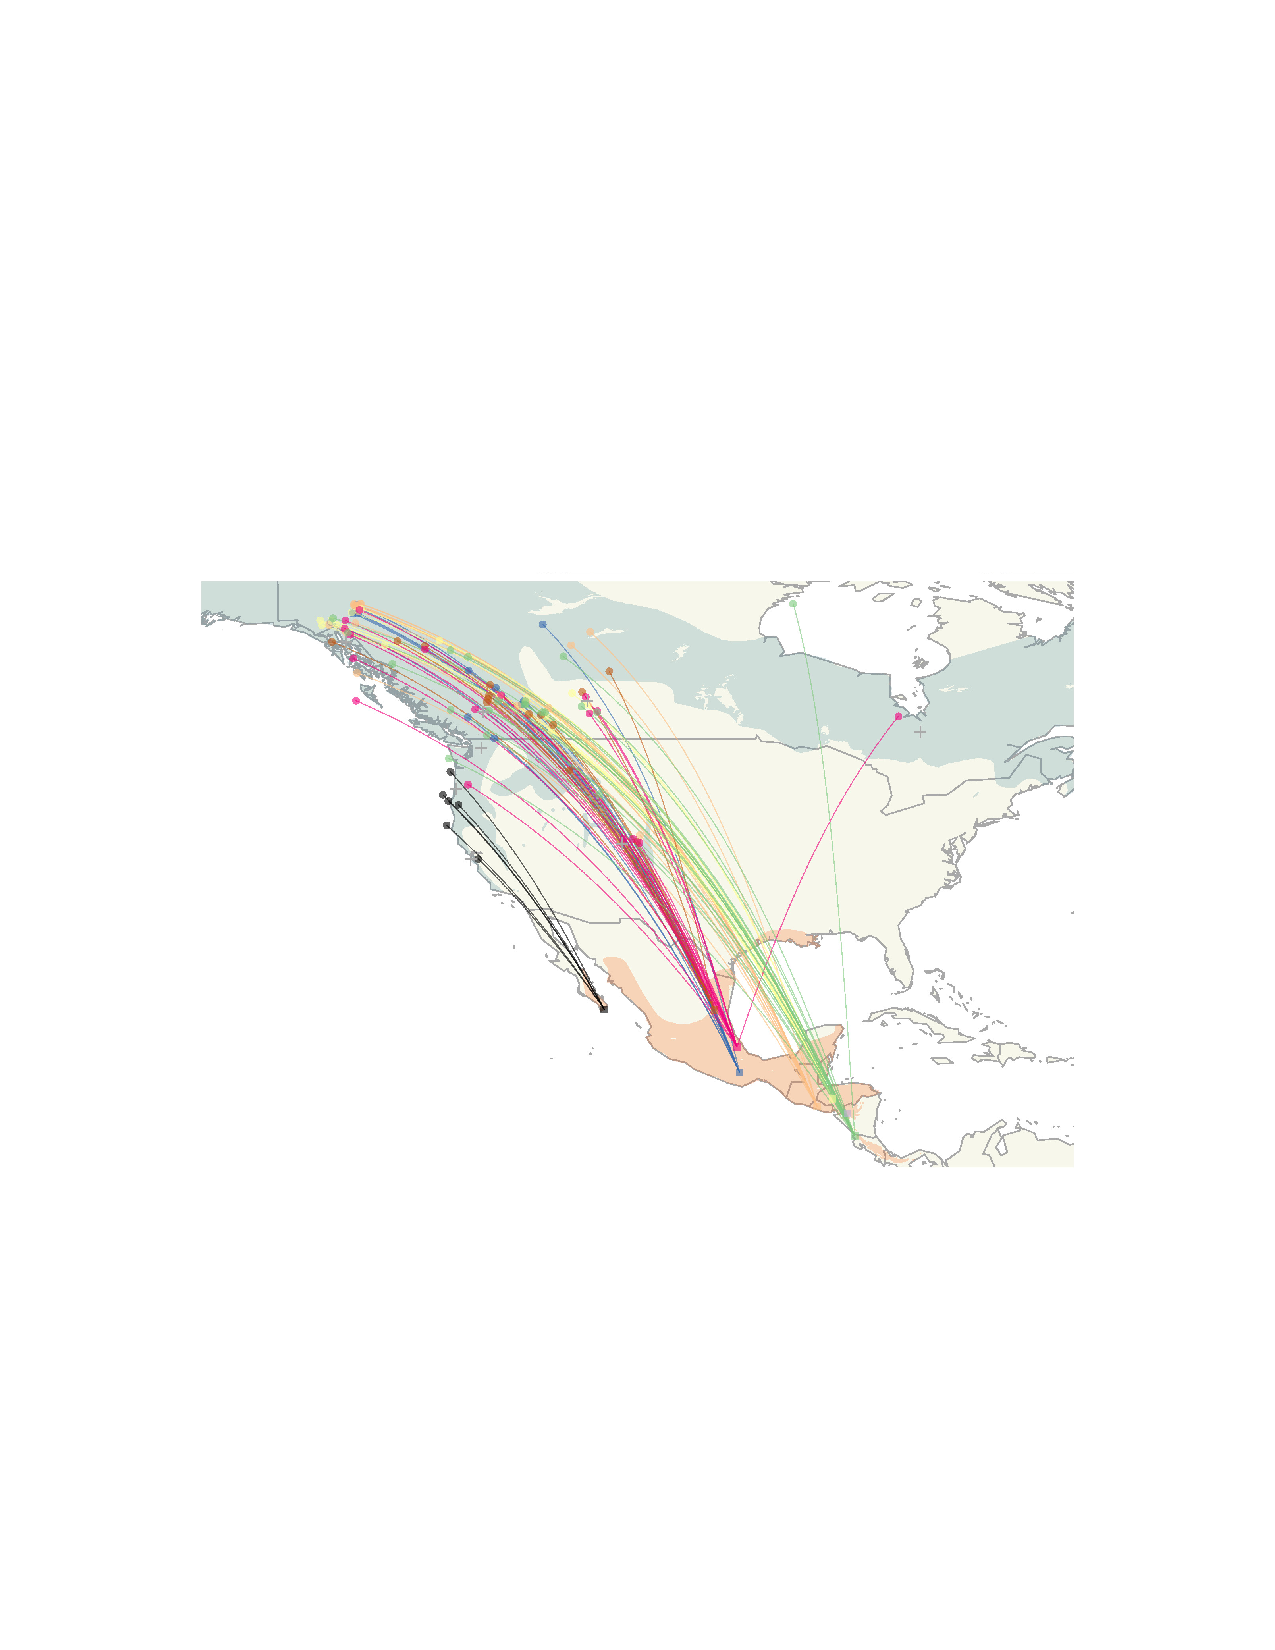
\includegraphics[width=0.9\textwidth]{figs/wintering.pdf}
\end{center}

\end{frame}

\end{document}
